\chapter*{More figures}
\addcontentsline{toc}{chapter}{More figures}

Some figures are referred to in the text but not placed directly under the text. These are included in this list. All figures are high resolution thus zooming in the PDF should be viable to get a clearer view.

%------------------------------------

\section*{Overview of training set}

\begin{figure}[H]
    \begin{center}
        \fbox{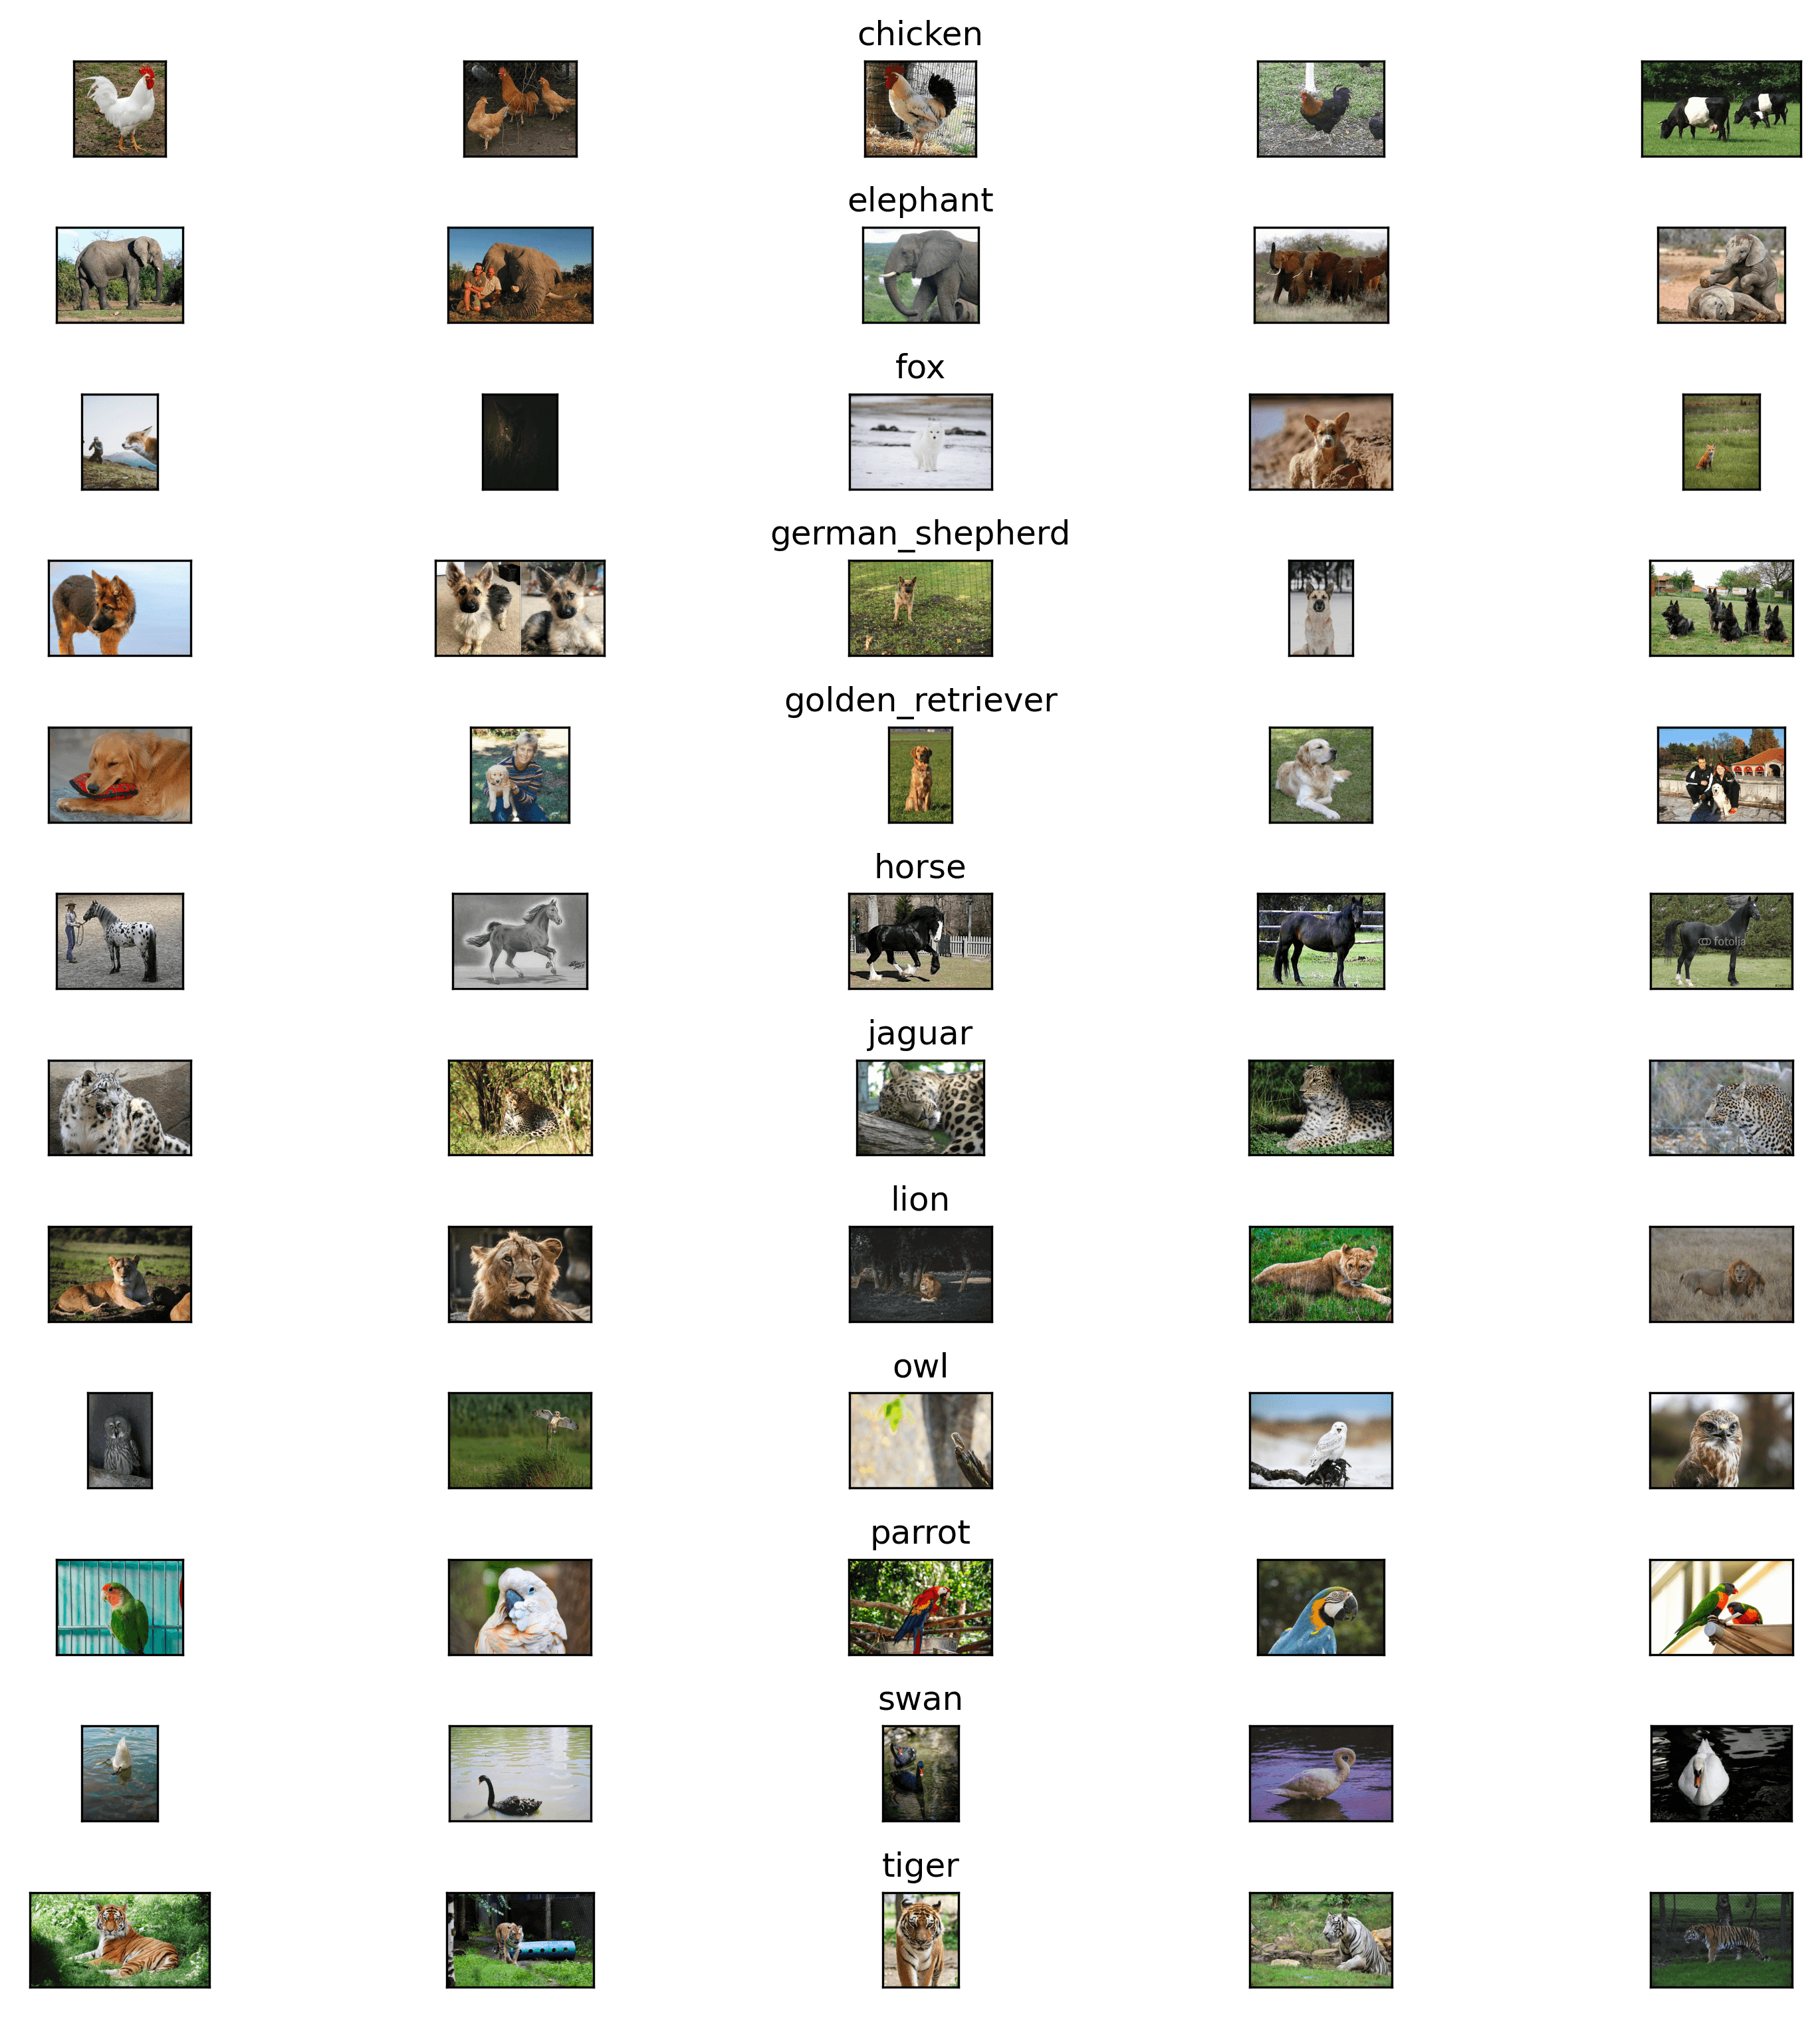
\includegraphics[width=0.6\linewidth]{images/1/1-data_analysis-labeled_data_overview.png}}
    \end{center}
    \captionsetup{width=0.65\linewidth}
    \captionsetup{justification=centering}
    \caption{An overview of the supplied data per class.}
    \label{fig:1-data_analysis-labeled_data_overview.png}
\end{figure}

%------------------------------------

\section*{Learning curves of the models}

\begin{figure}[H]
    \centering
    \fbox{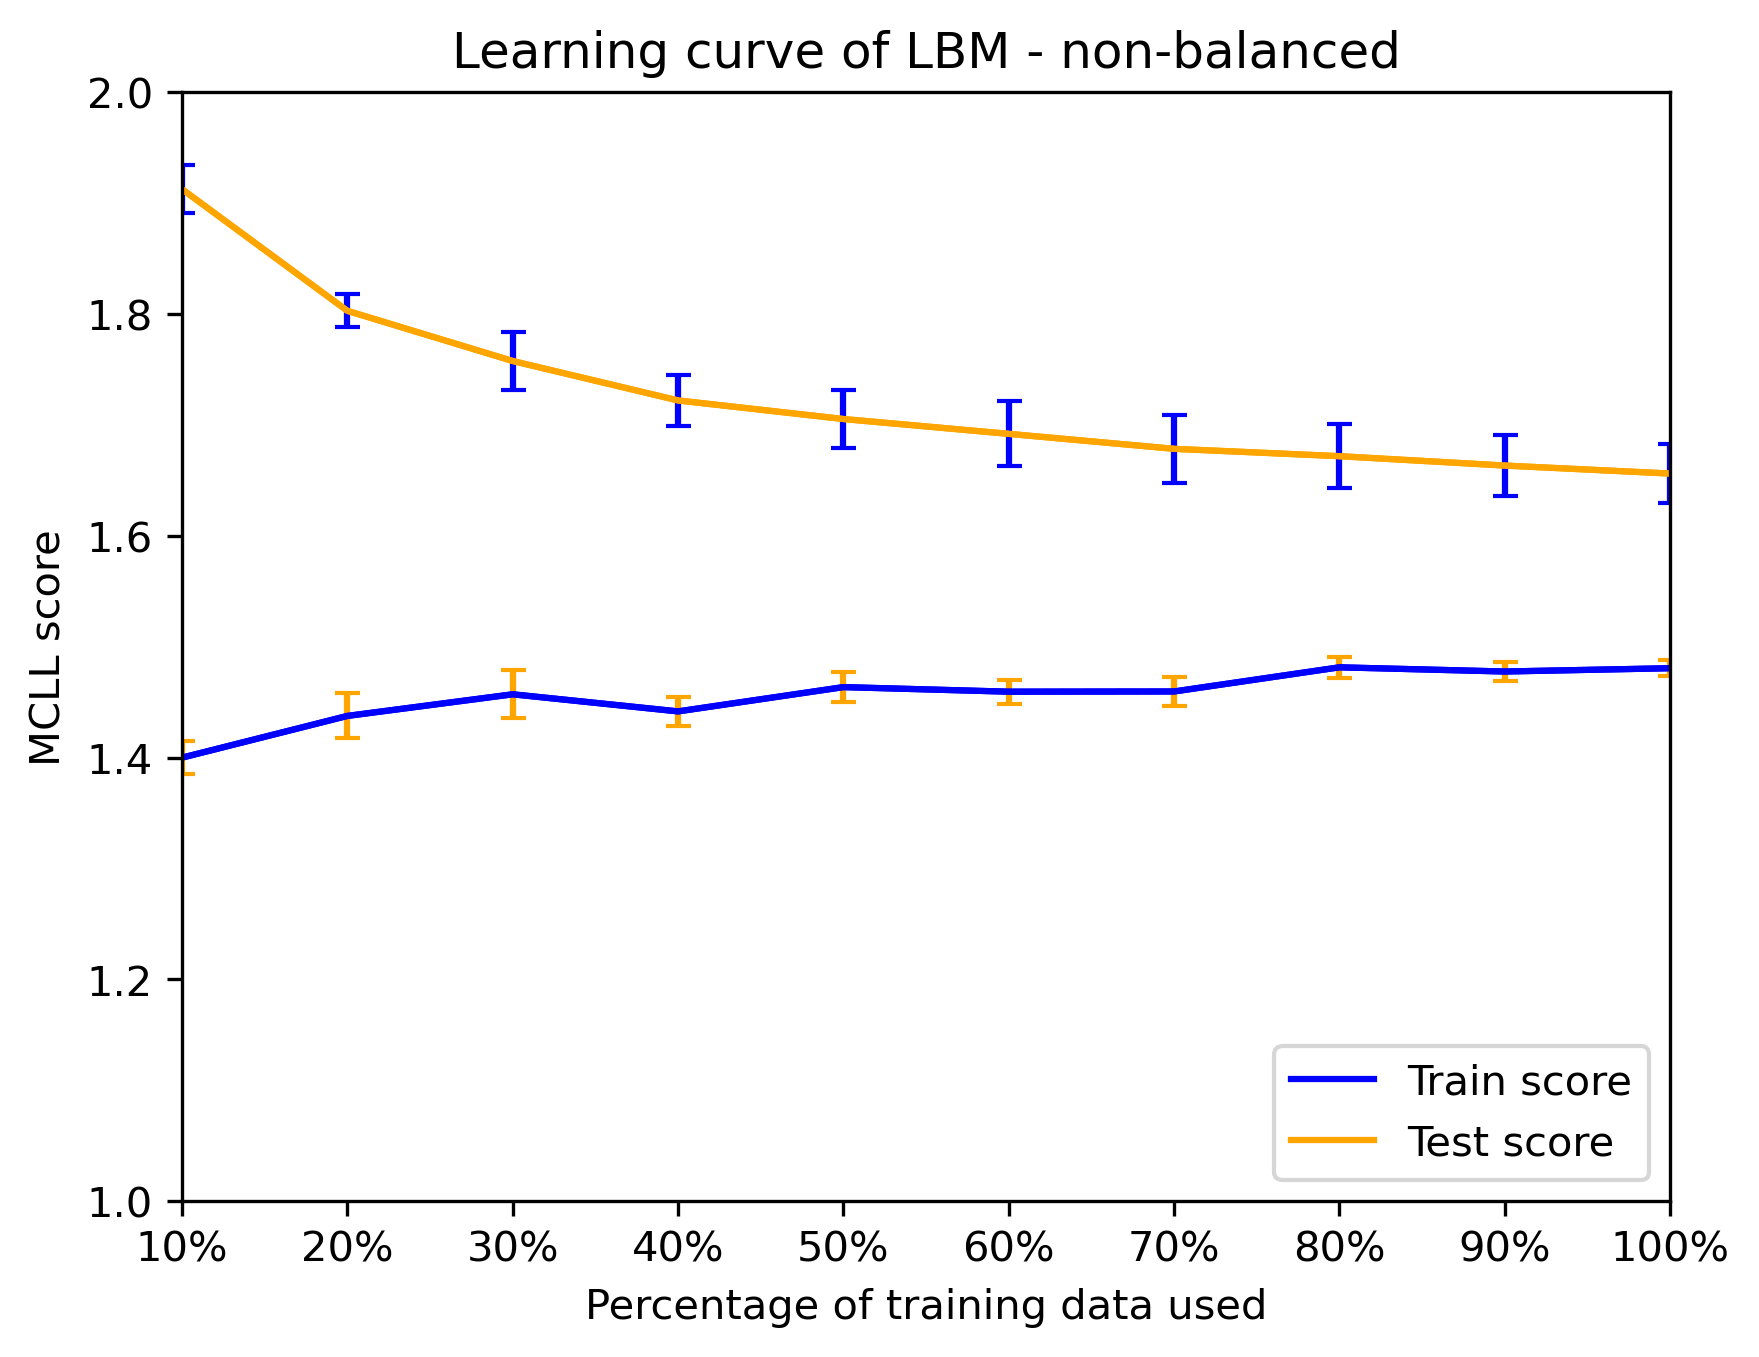
\includegraphics[width=0.65\linewidth]{images/MA/MA_LBM_learning_curve.png}}
    \captionsetup{width=0.6\linewidth}
    \captionsetup{justification=centering}
    \caption{Learning curve of the non-balanced linear baseline model.}
\end{figure}

\begin{figure}[H]
    \centering
    \fbox{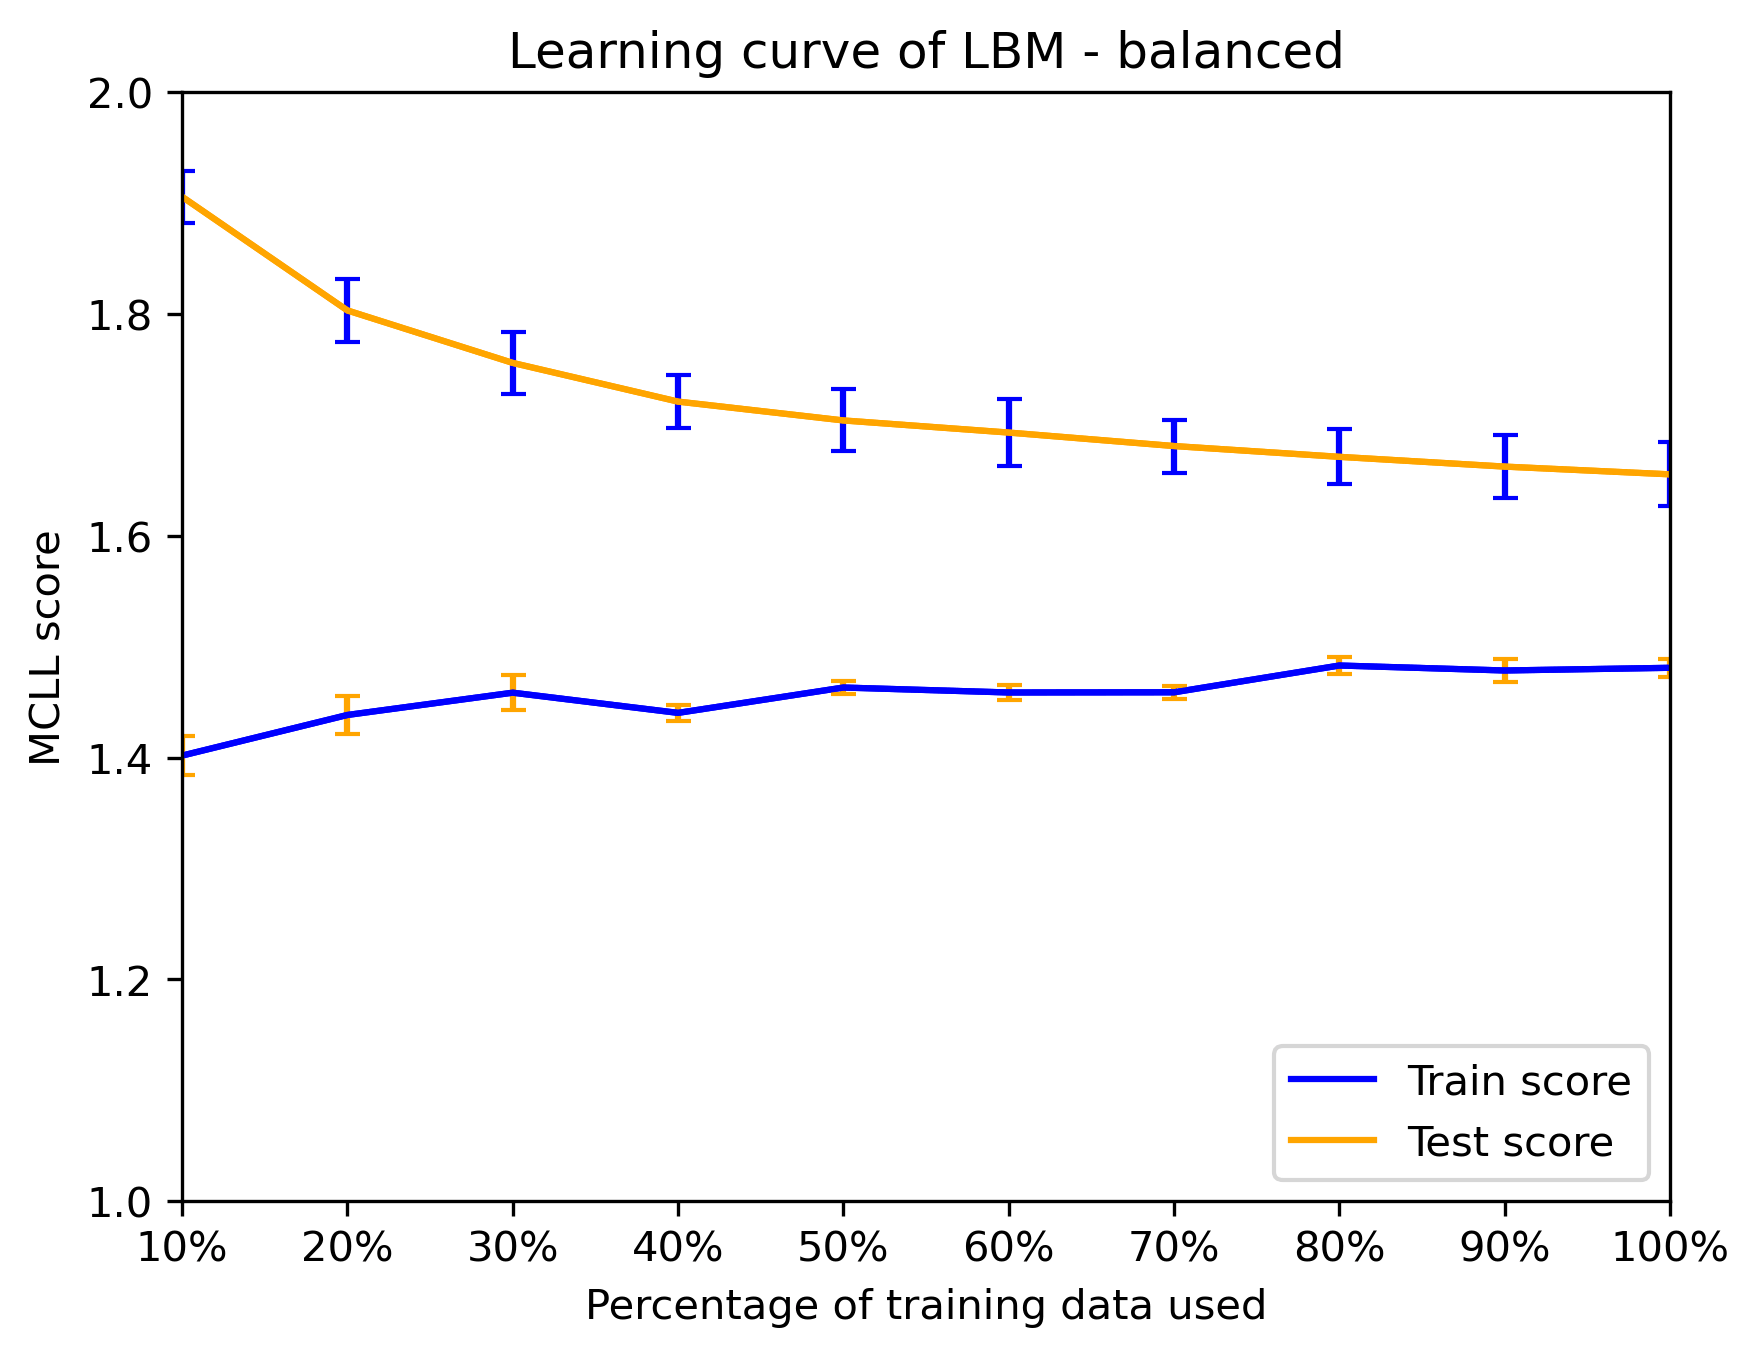
\includegraphics[width=0.65\linewidth]{images/MA/MA_LBM_learning_curve_balanced.png}}
    \captionsetup{width=0.6\linewidth}
    \captionsetup{justification=centering}
    \caption{Learning curve of the balanced linear baseline model.}
\end{figure}

\begin{figure}[H]
    \centering
    \fbox{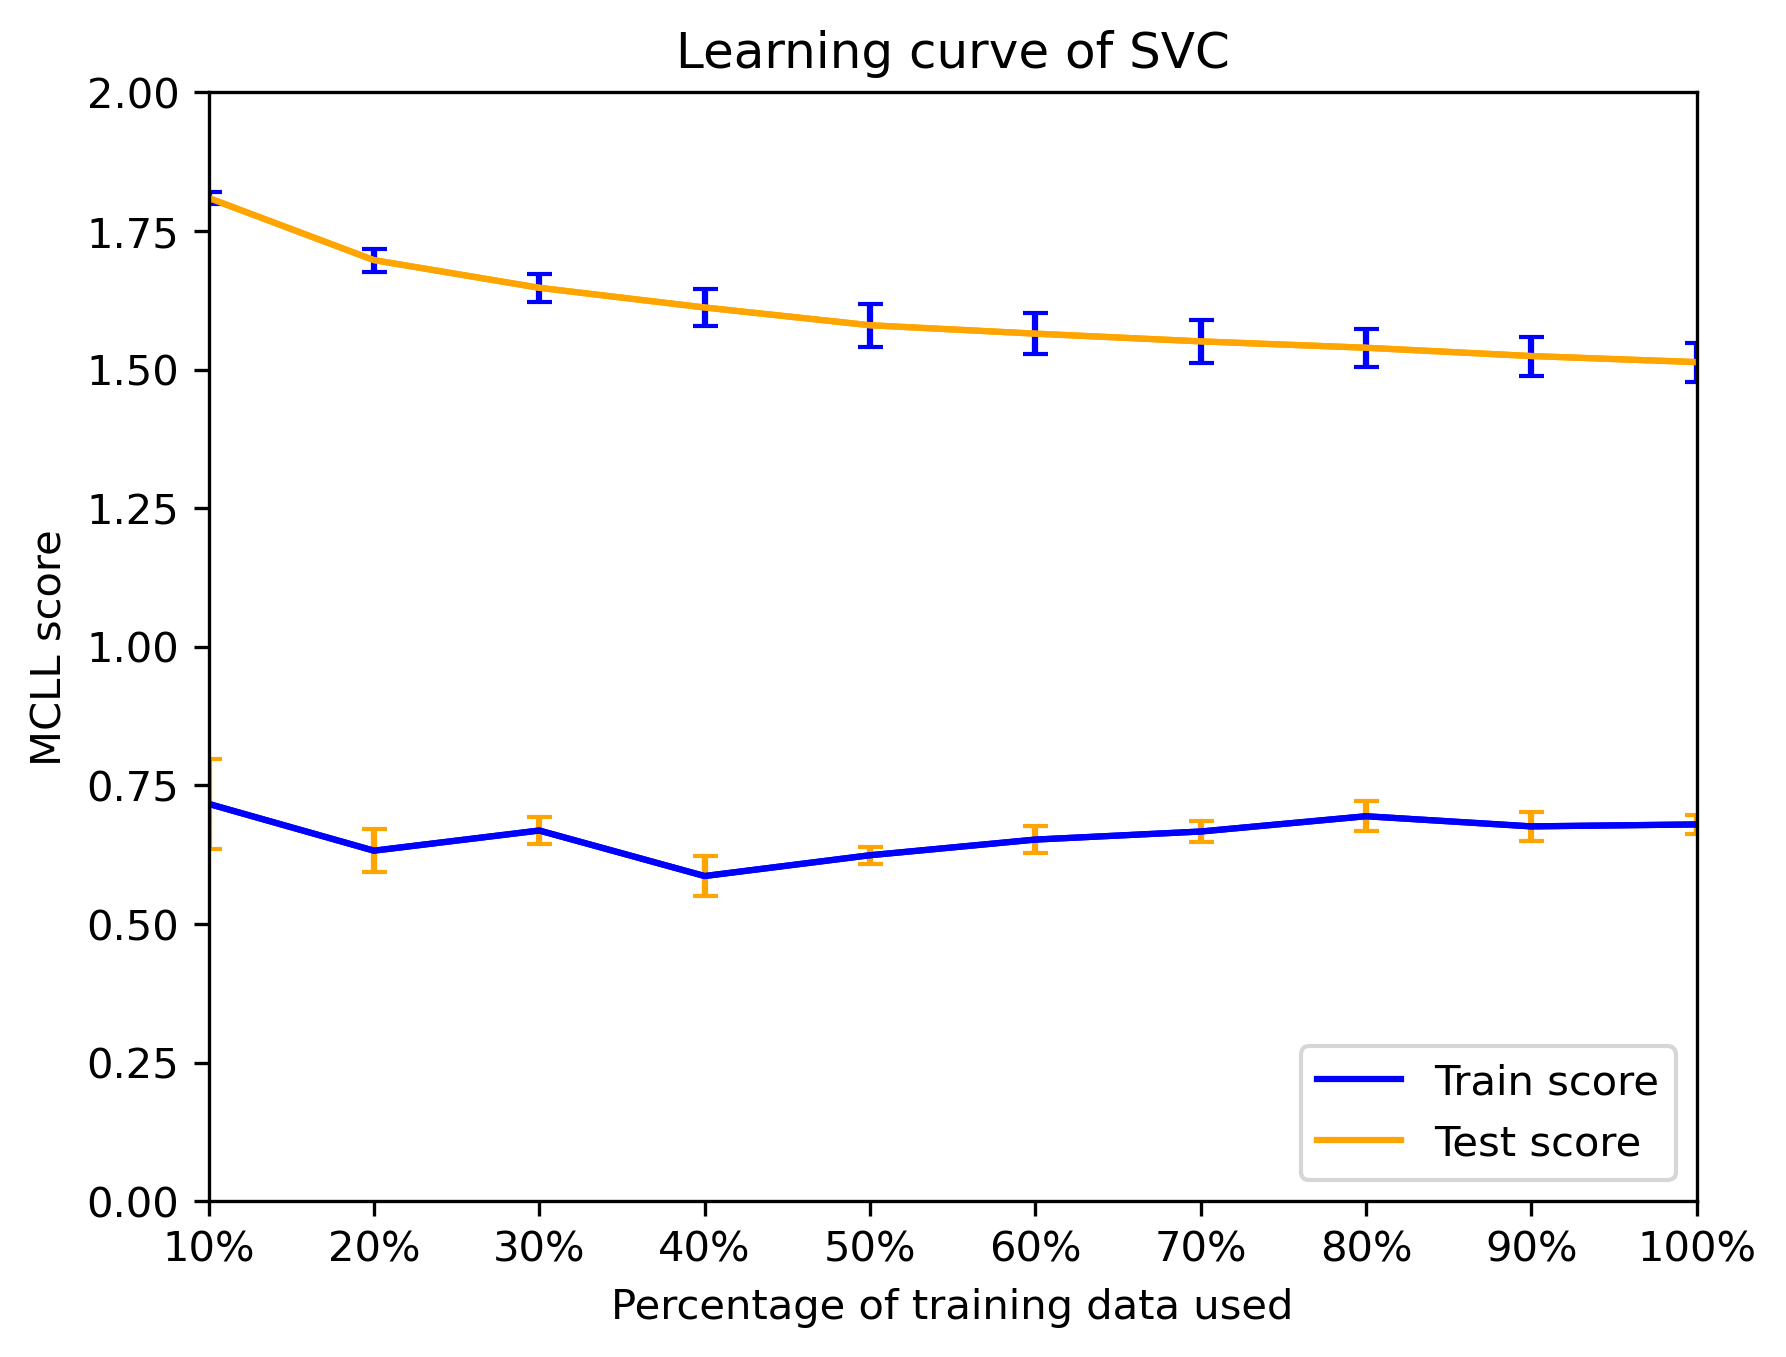
\includegraphics[width=0.75\linewidth]{images/MA/MA_SVC_learning_curve.png}}
    \captionsetup{width=0.7\linewidth}
    \captionsetup{justification=centering}
    \caption{Learning curve of the SVC model.}
\end{figure}

\begin{figure}[H]
    \centering
    \fbox{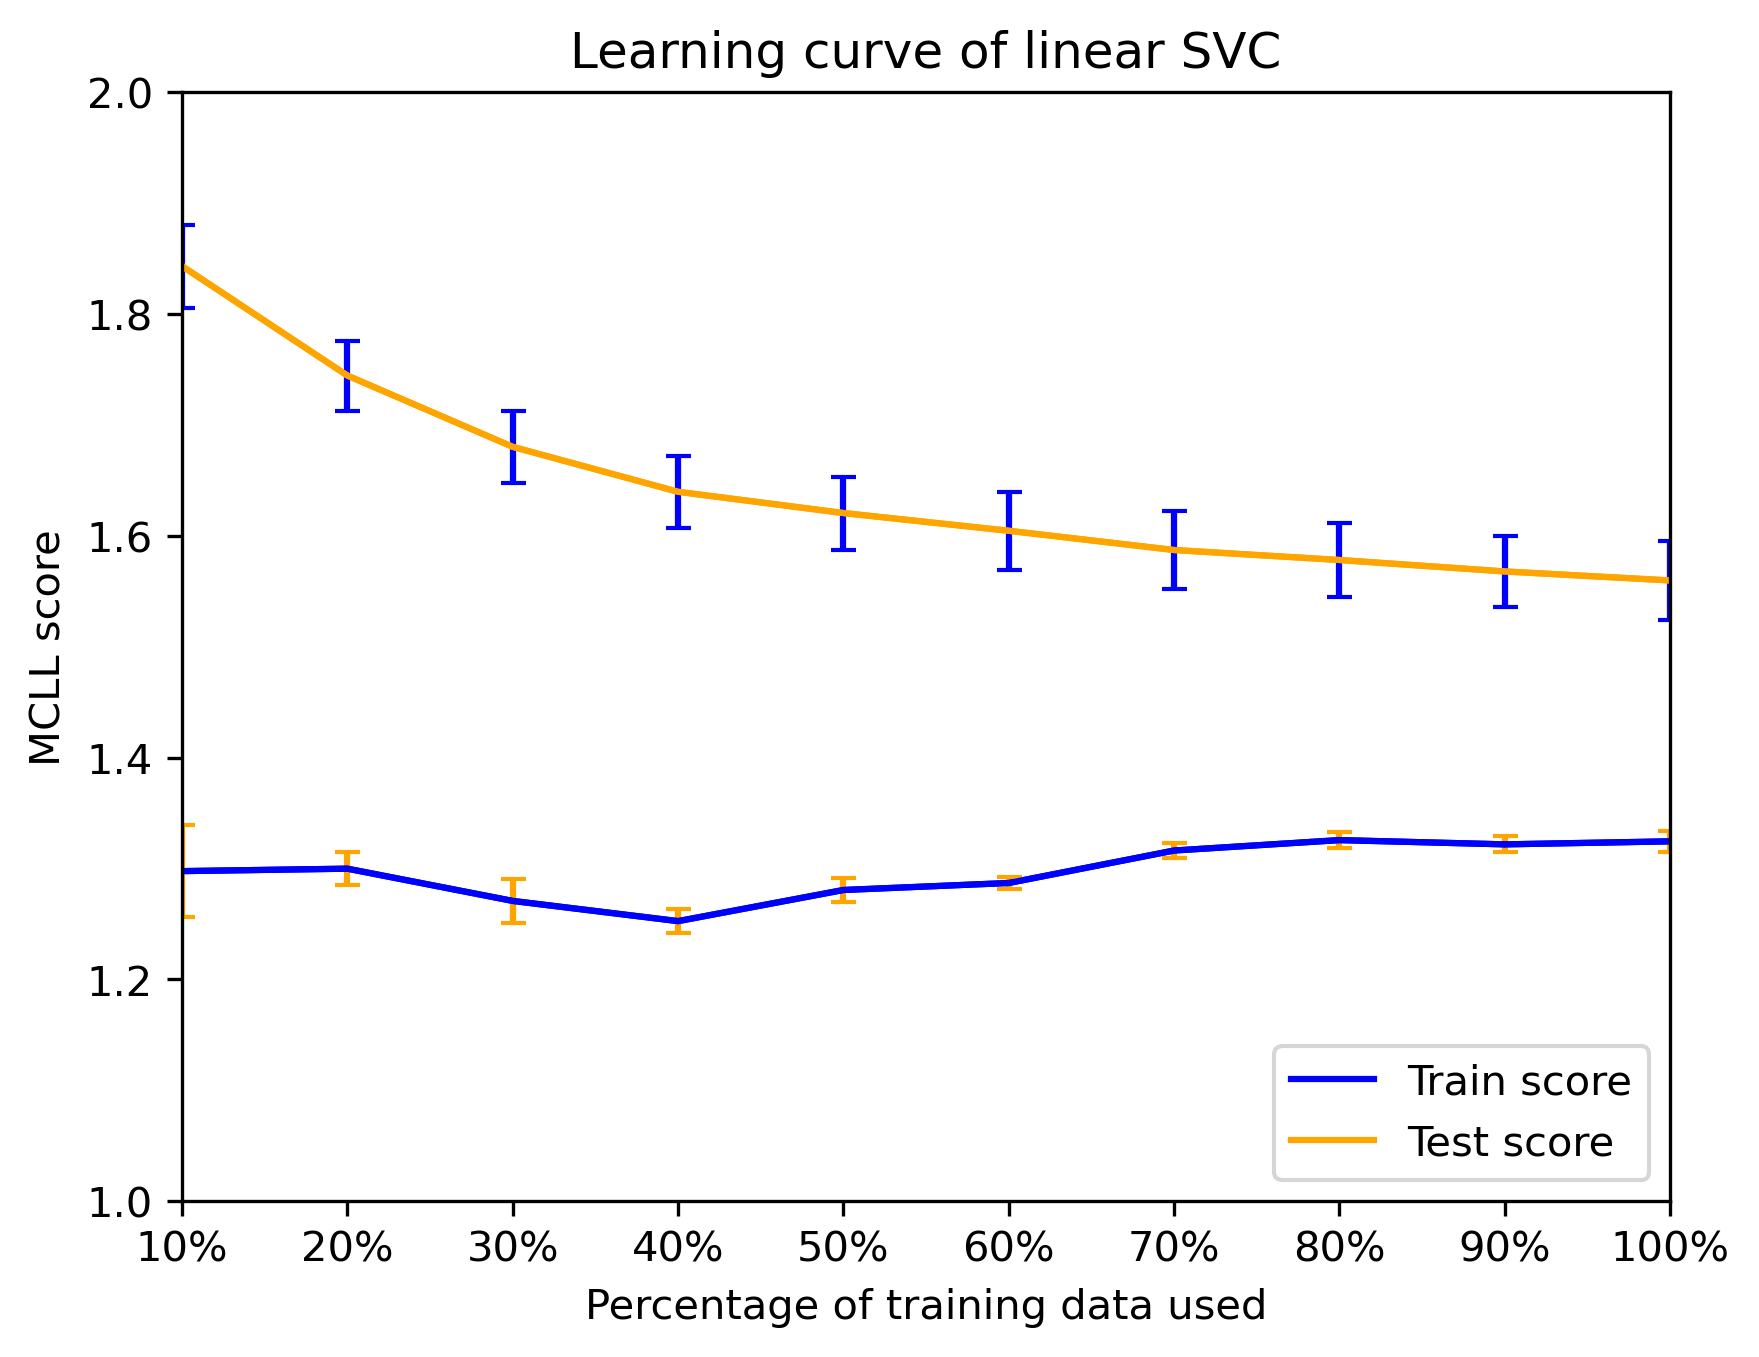
\includegraphics[width=0.75\linewidth]{images/MA/MA_linSVC_learning_curve.png}}
    \captionsetup{width=0.7\linewidth}
    \captionsetup{justification=centering}
    \caption{Learning curve of the linear SVC model.}
\end{figure}

%------------------------------------

\section*{Confusion matrix of linear SVC}

\begin{figure*}[ht]
    \centering
    \begin{subfigure}{.45\textwidth}
        \centering
        \fbox{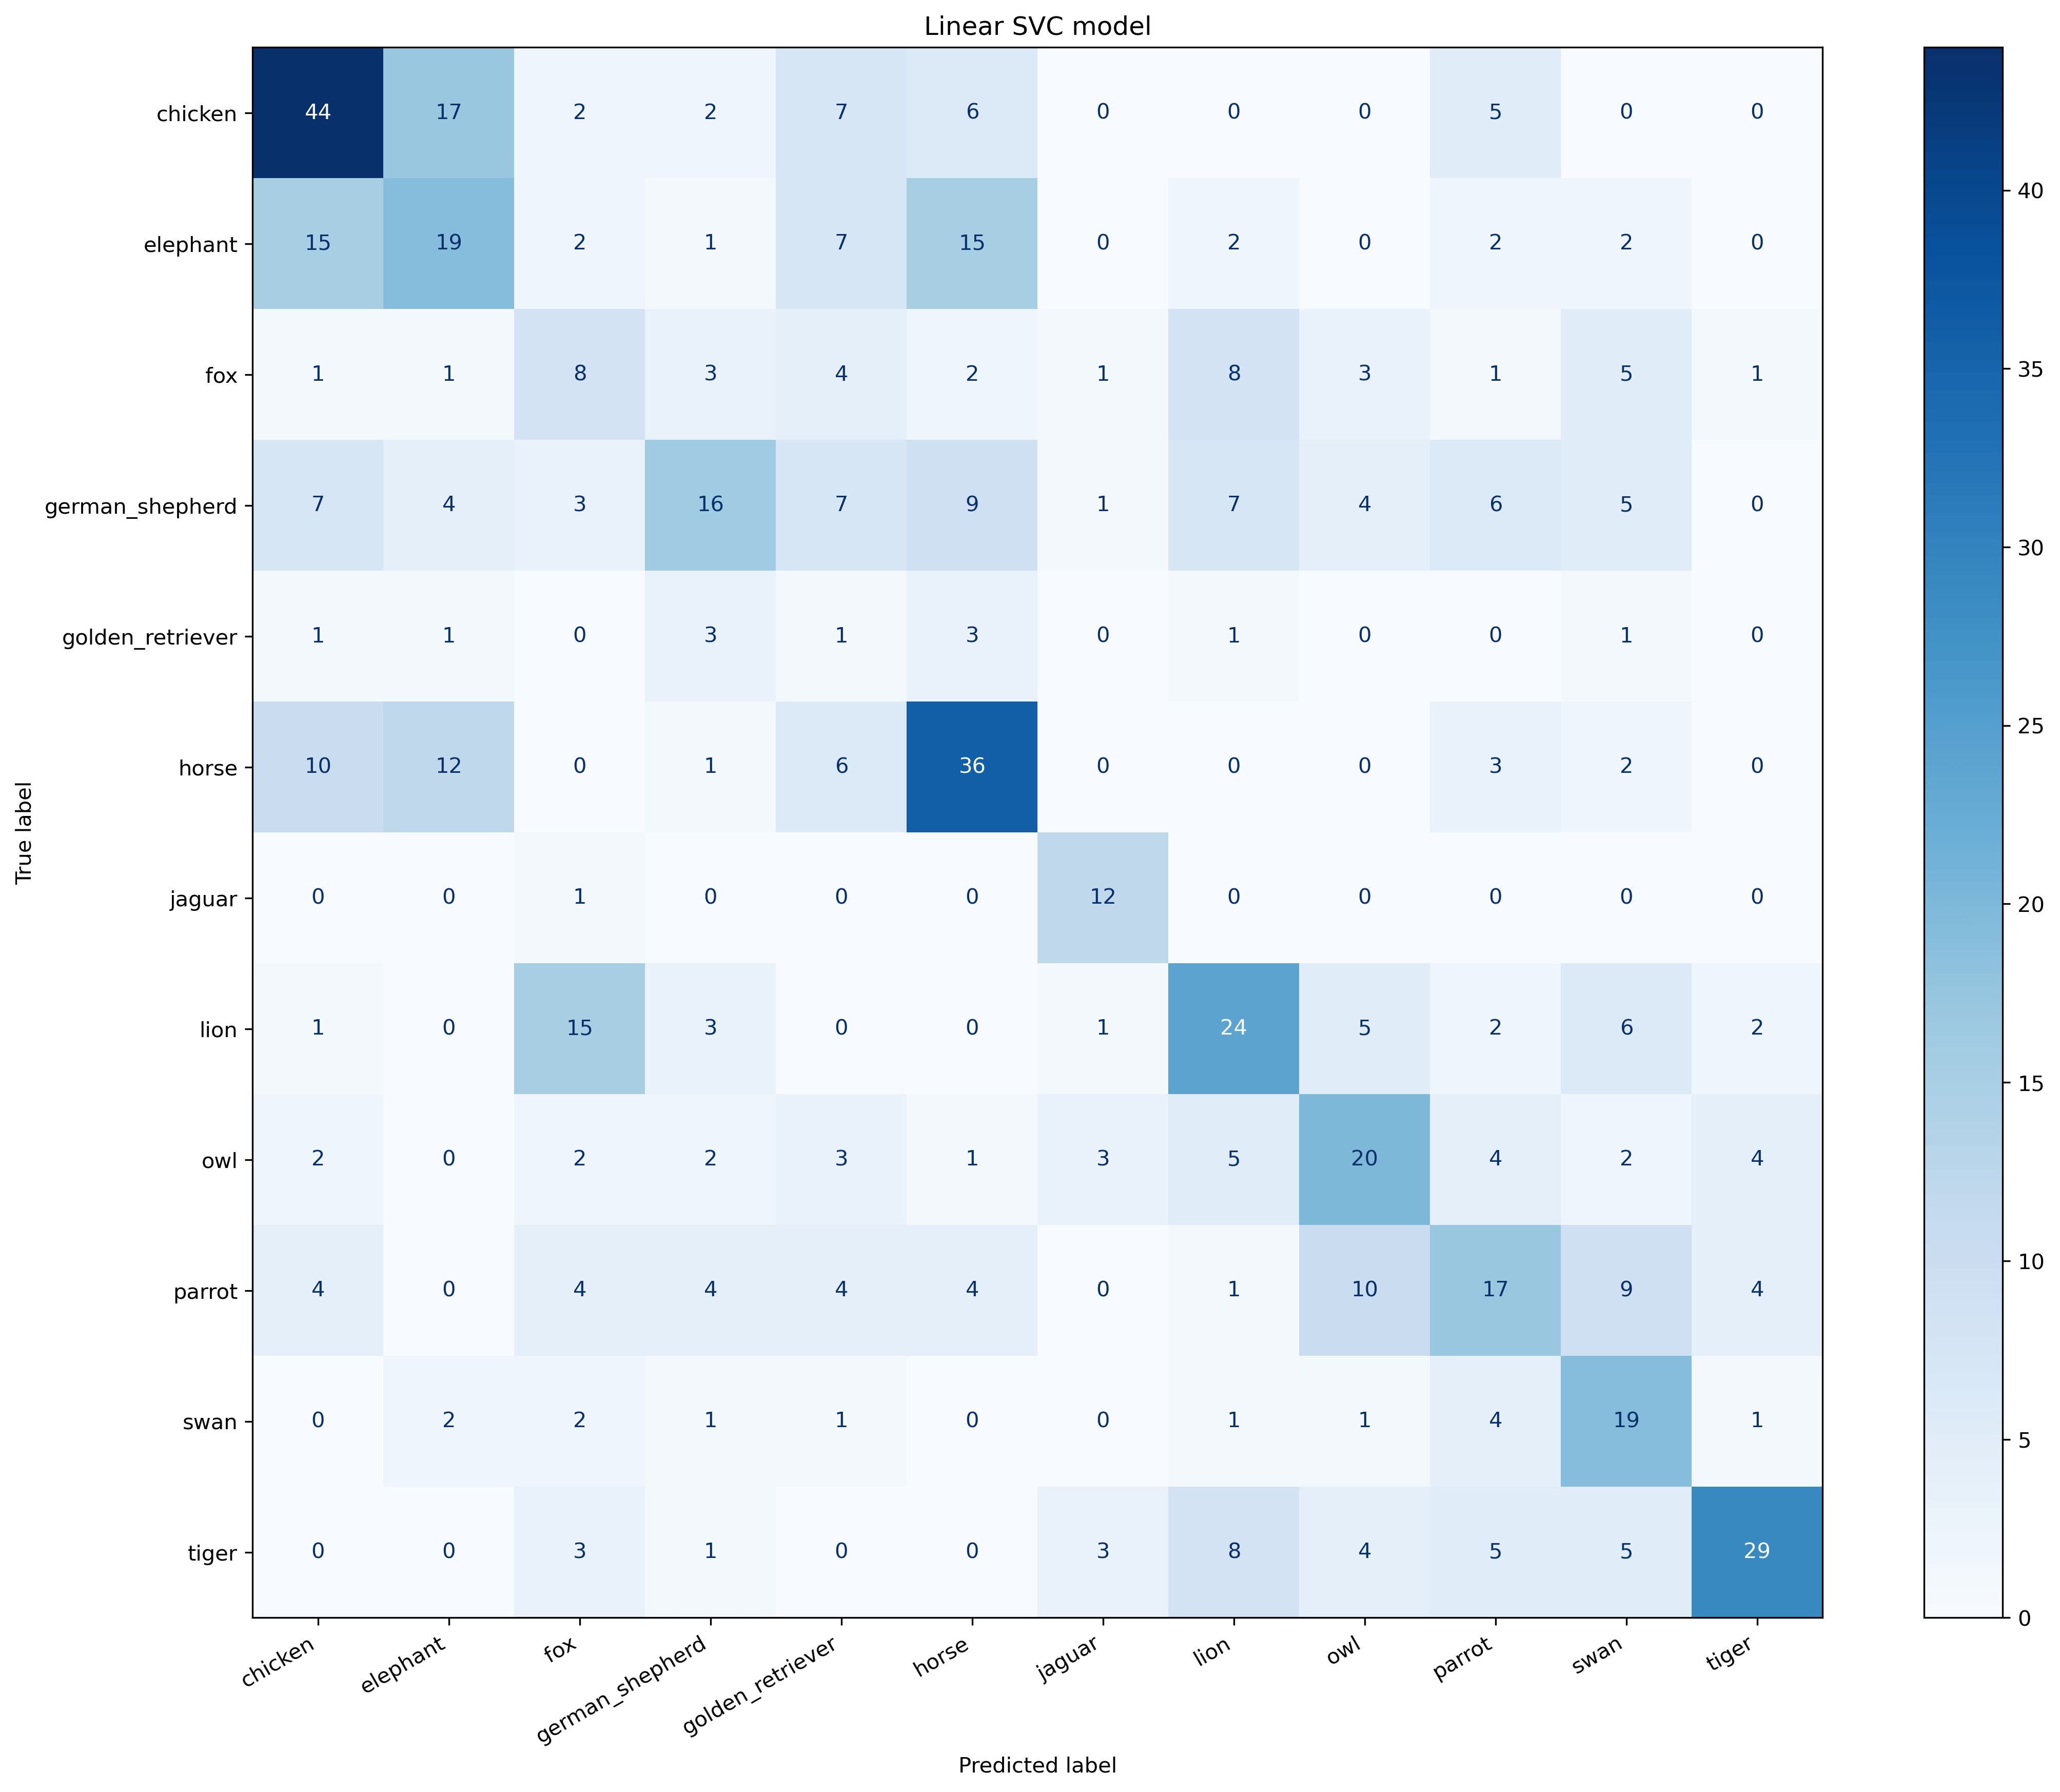
\includegraphics[width=\textwidth]{images/MA/MA_linSVC_non_normalised.png}}
        \captionsetup{width=0.9\linewidth}
        \captionsetup{justification=centering}
        \caption{Non normalised CM.}
    \end{subfigure}
    \hspace{1cm}
    \begin{subfigure}{.45\textwidth}
        \centering
        \fbox{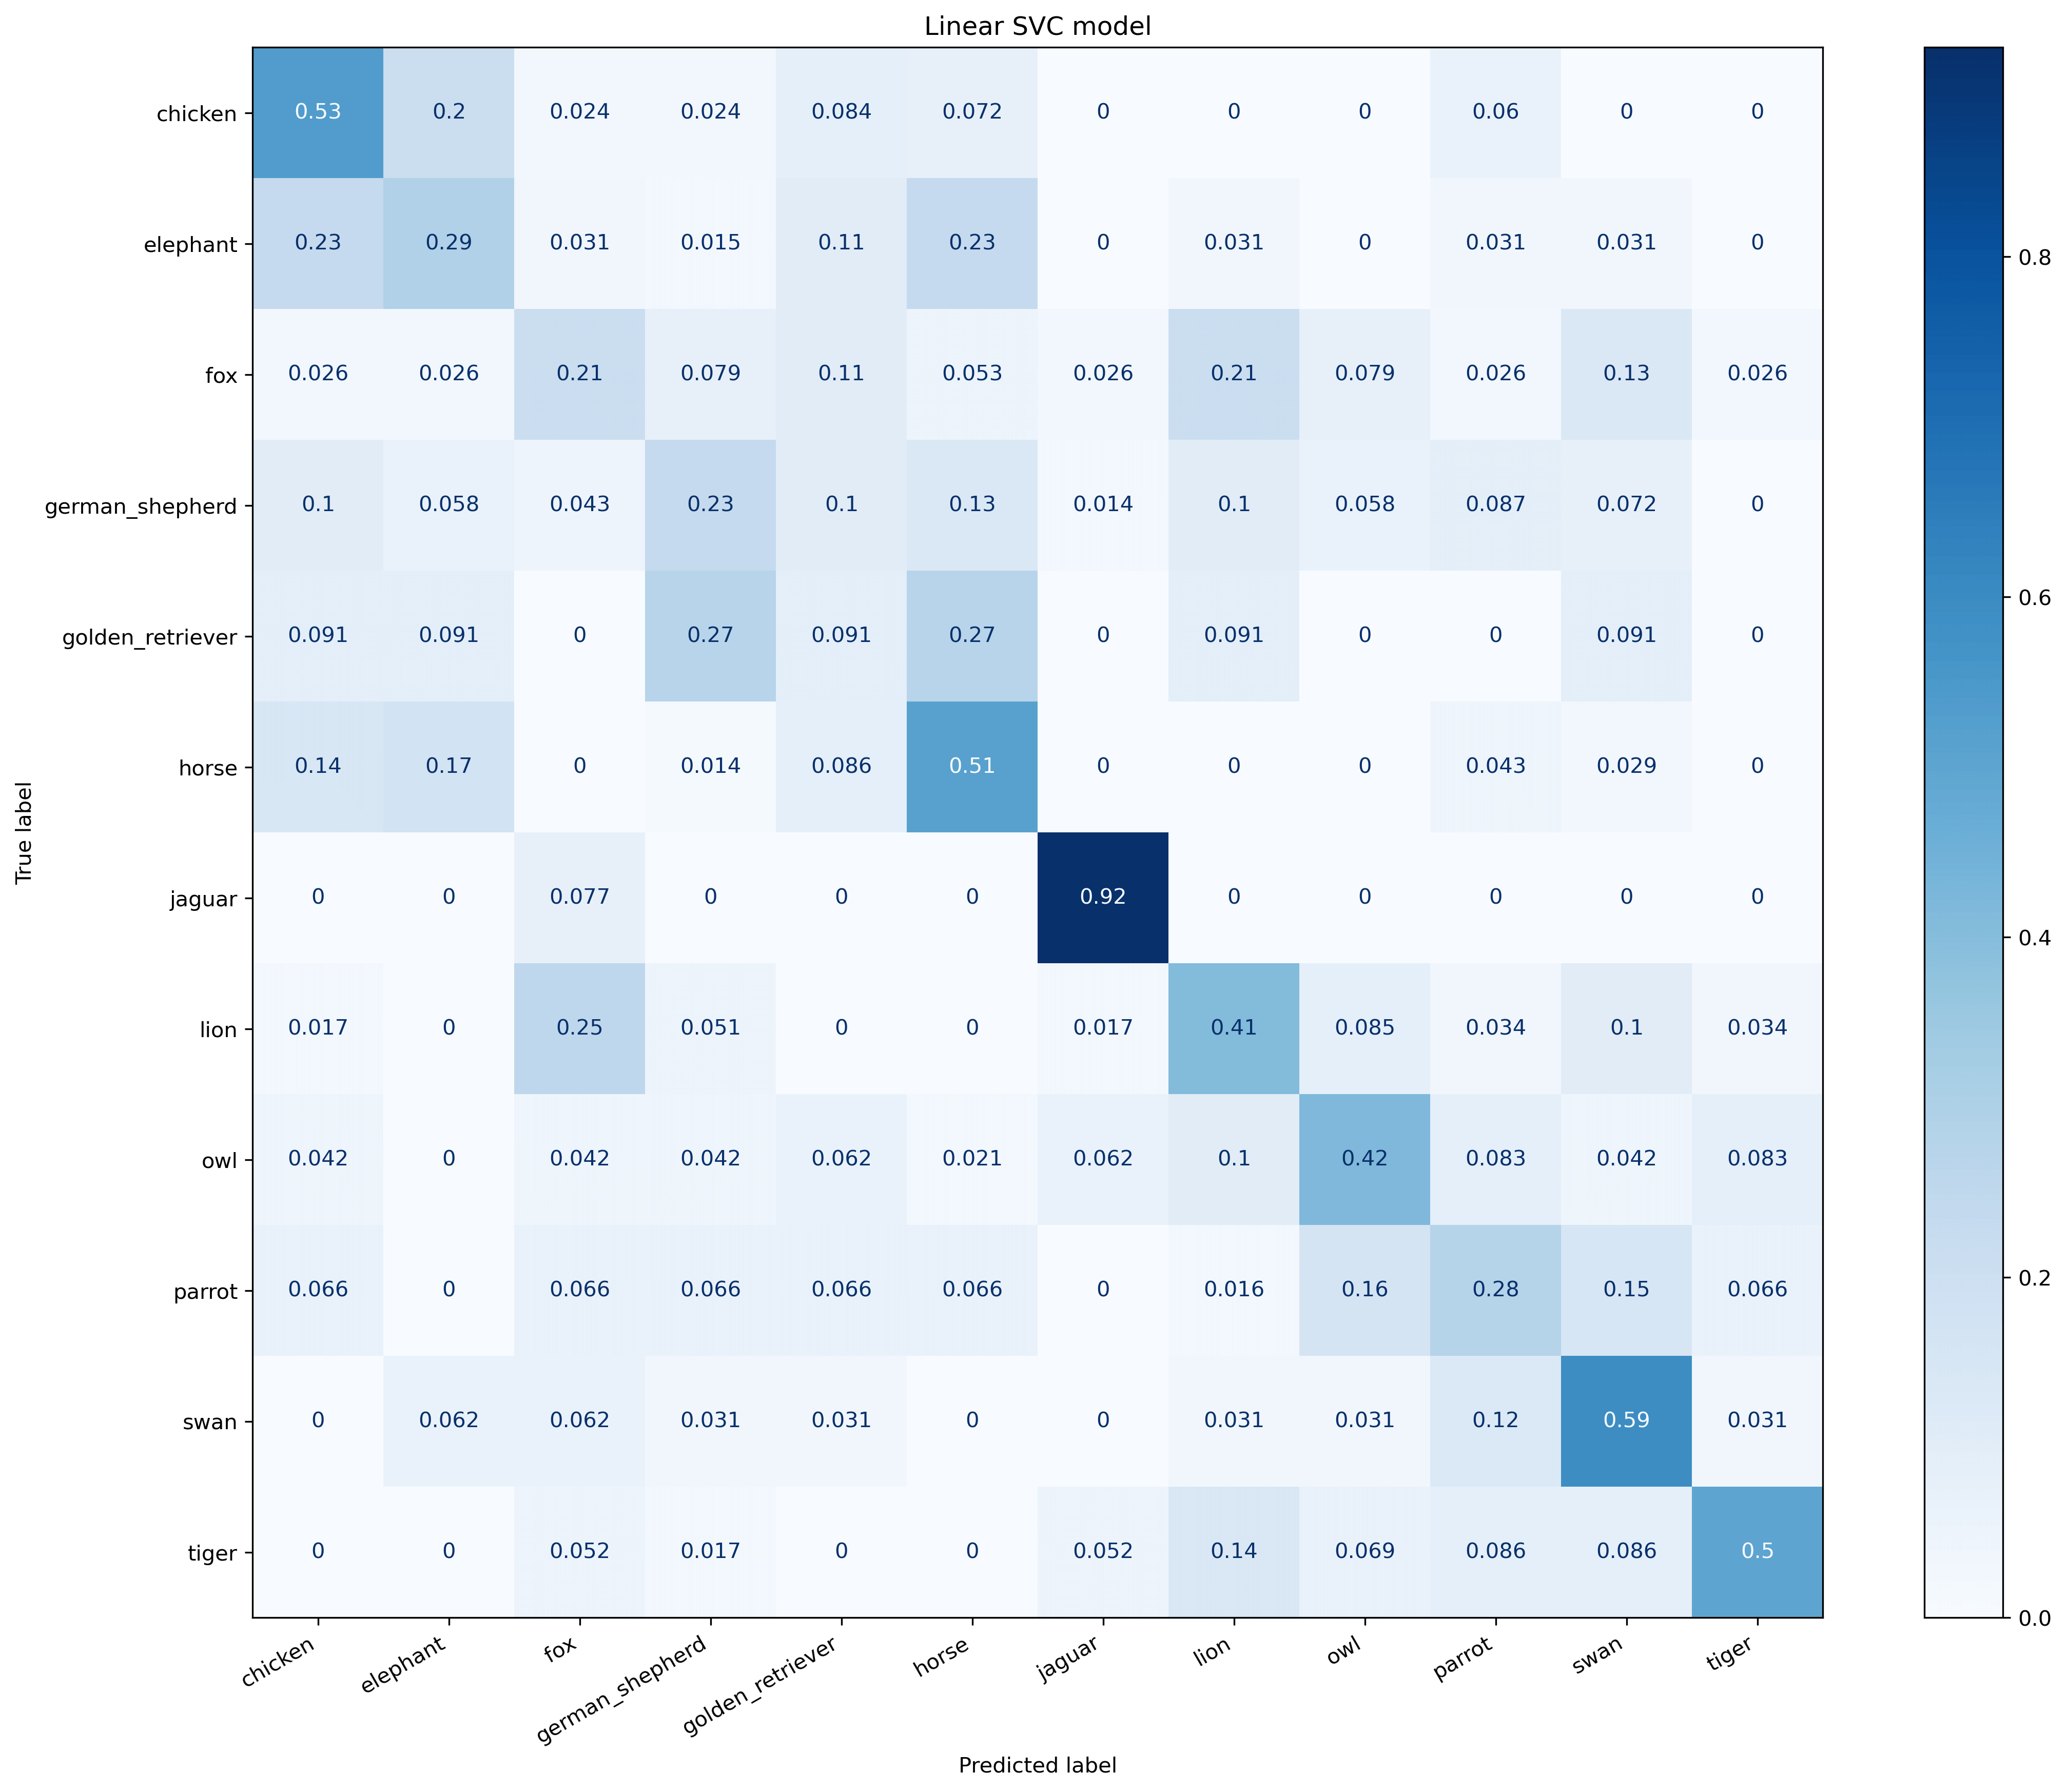
\includegraphics[width=\textwidth]{images/MA/MA_linSVC_normalised.png}}
        \captionsetup{width=0.9\linewidth}
        \captionsetup{justification=centering}
        \caption{Normalised CM.}
    \end{subfigure}
    \captionsetup{width=0.9\linewidth}
    \captionsetup{justification=centering}
    \caption{Confusion matrices for the linear Support Vector Classifier model.}
    \label{fig:ma_linsvc_cm}
\end{figure*}



%------------------------------------
\clearpage
\section*{Confusion matrices of the final model's underlying models}

\begin{figure*}[ht]
    \centering
    \begin{subfigure}{.45\textwidth}
        \centering
        \fbox{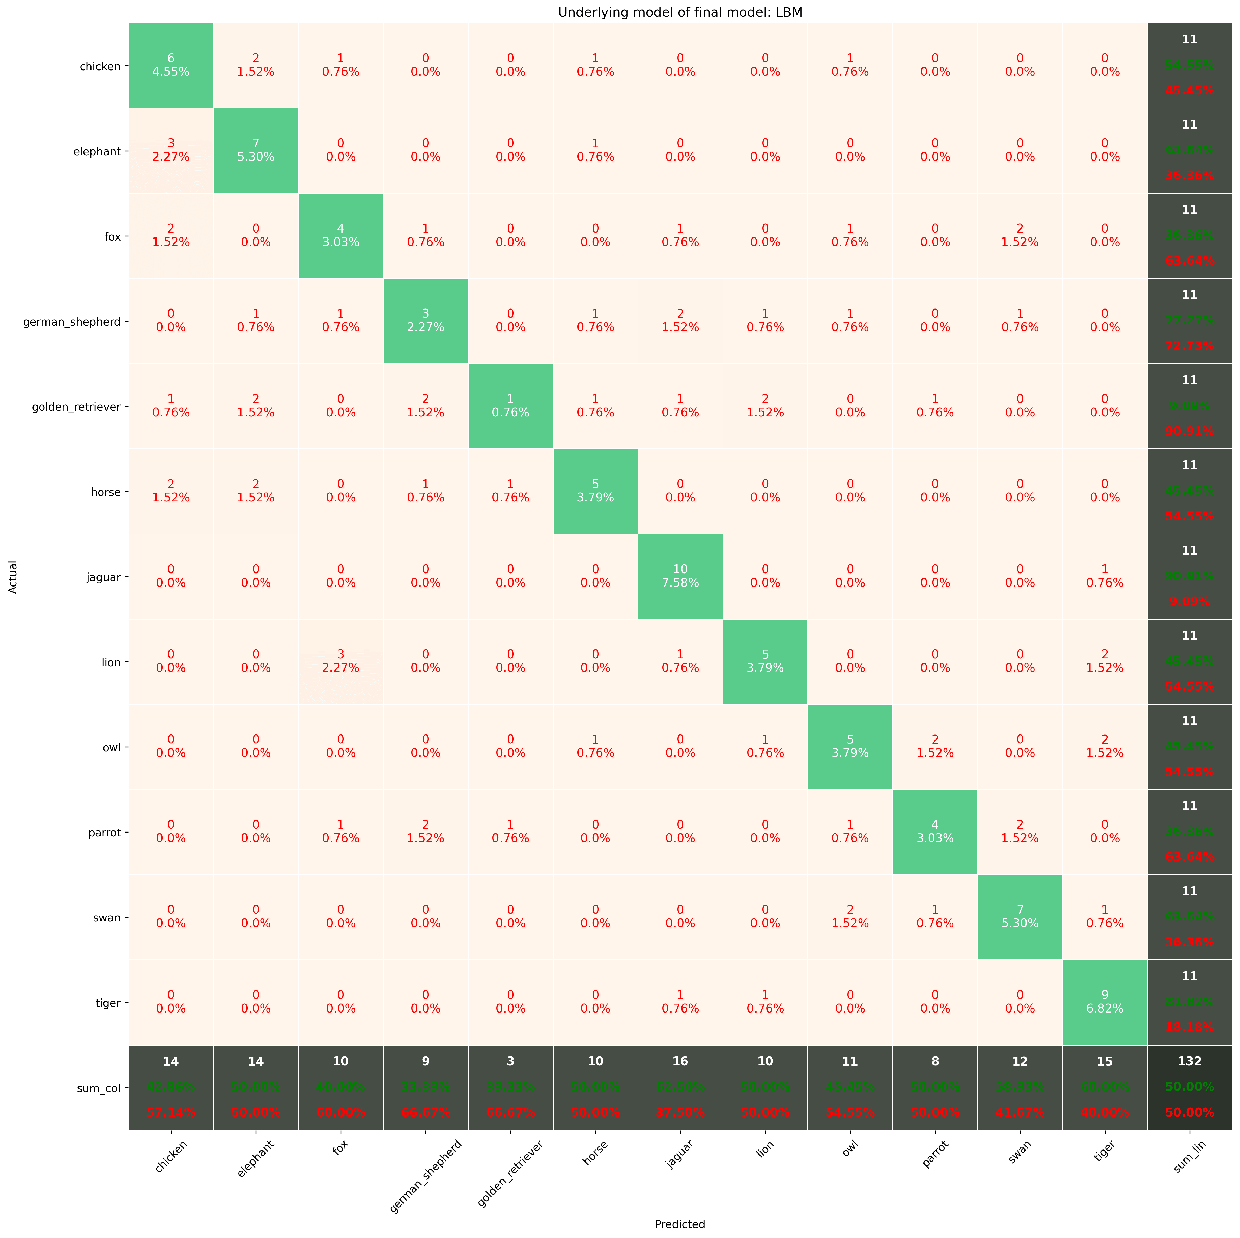
\includegraphics[width=\textwidth]{images/final/cm/underlying_LBM.pdf}}
        \captionsetup{width=0.8\linewidth}
        \captionsetup{justification=centering}
        \caption{Underlying LBM model.}
    \end{subfigure}
    \hspace{1cm}
    \begin{subfigure}{.45\textwidth}
        \centering
        \fbox{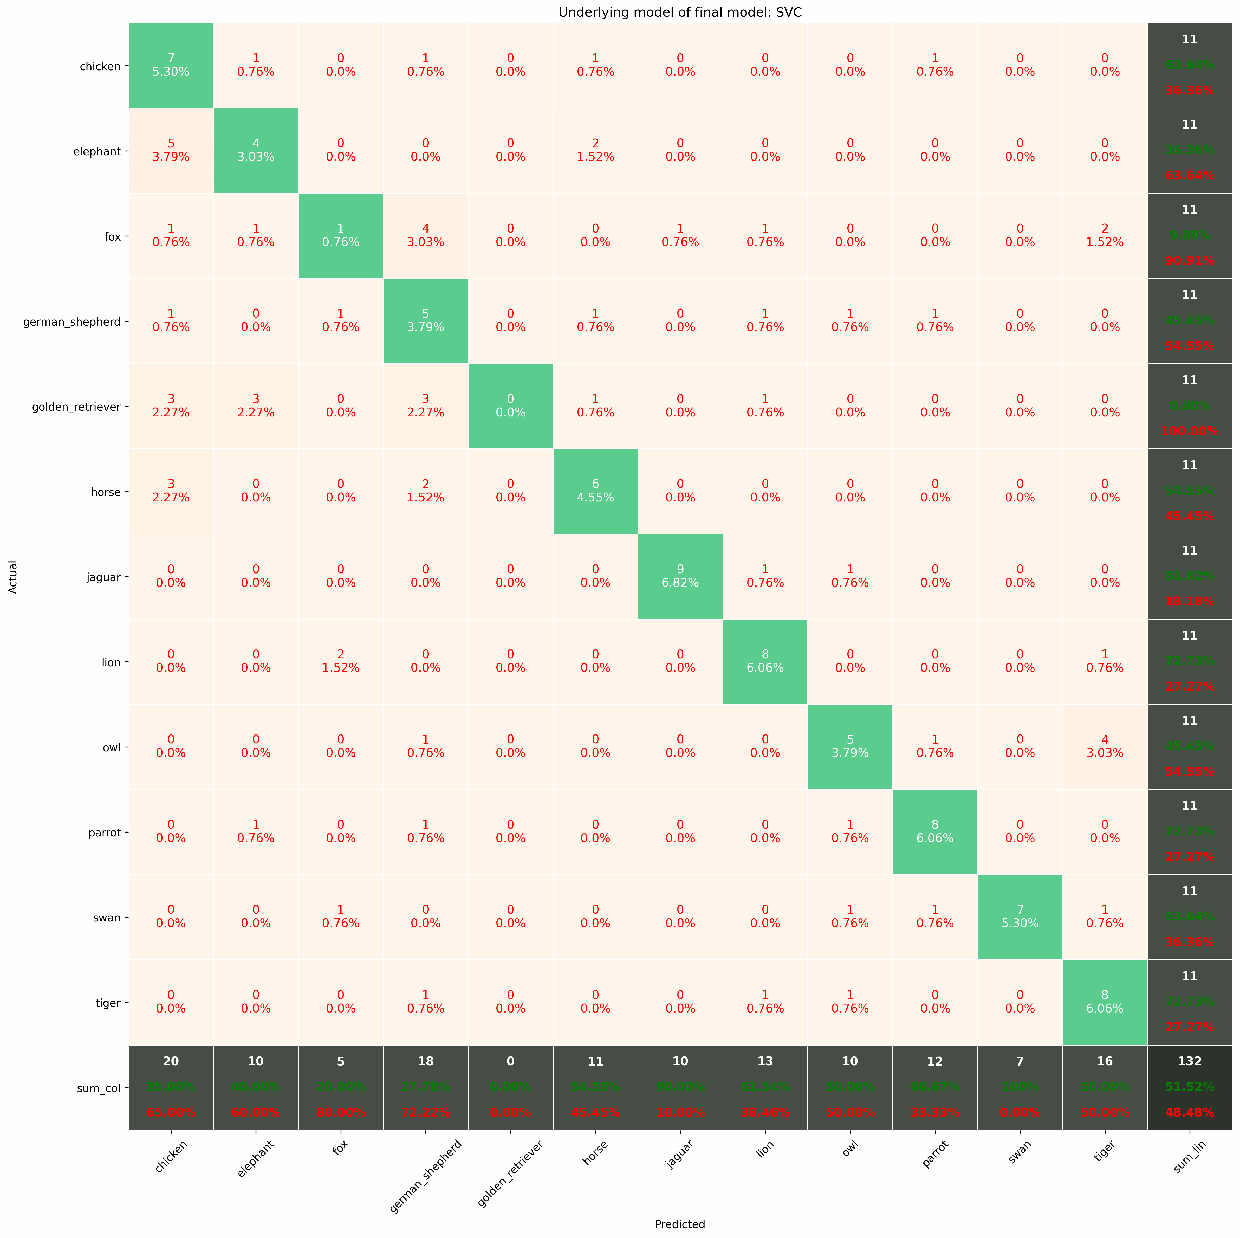
\includegraphics[width=\textwidth]{images/final/cm/underlying_SVC.pdf}}
        \captionsetup{width=0.8\linewidth}
        \captionsetup{justification=centering}
        \caption{Underlying SVC model.}
    \end{subfigure}
    \captionsetup{width=0.9\linewidth}
    \captionsetup{justification=centering}
    \caption{Underlying models of the final model using the complete data set.}
\end{figure*}

\begin{figure*}[ht]
    \centering
    \begin{subfigure}{.45\textwidth}
        \centering
        \fbox{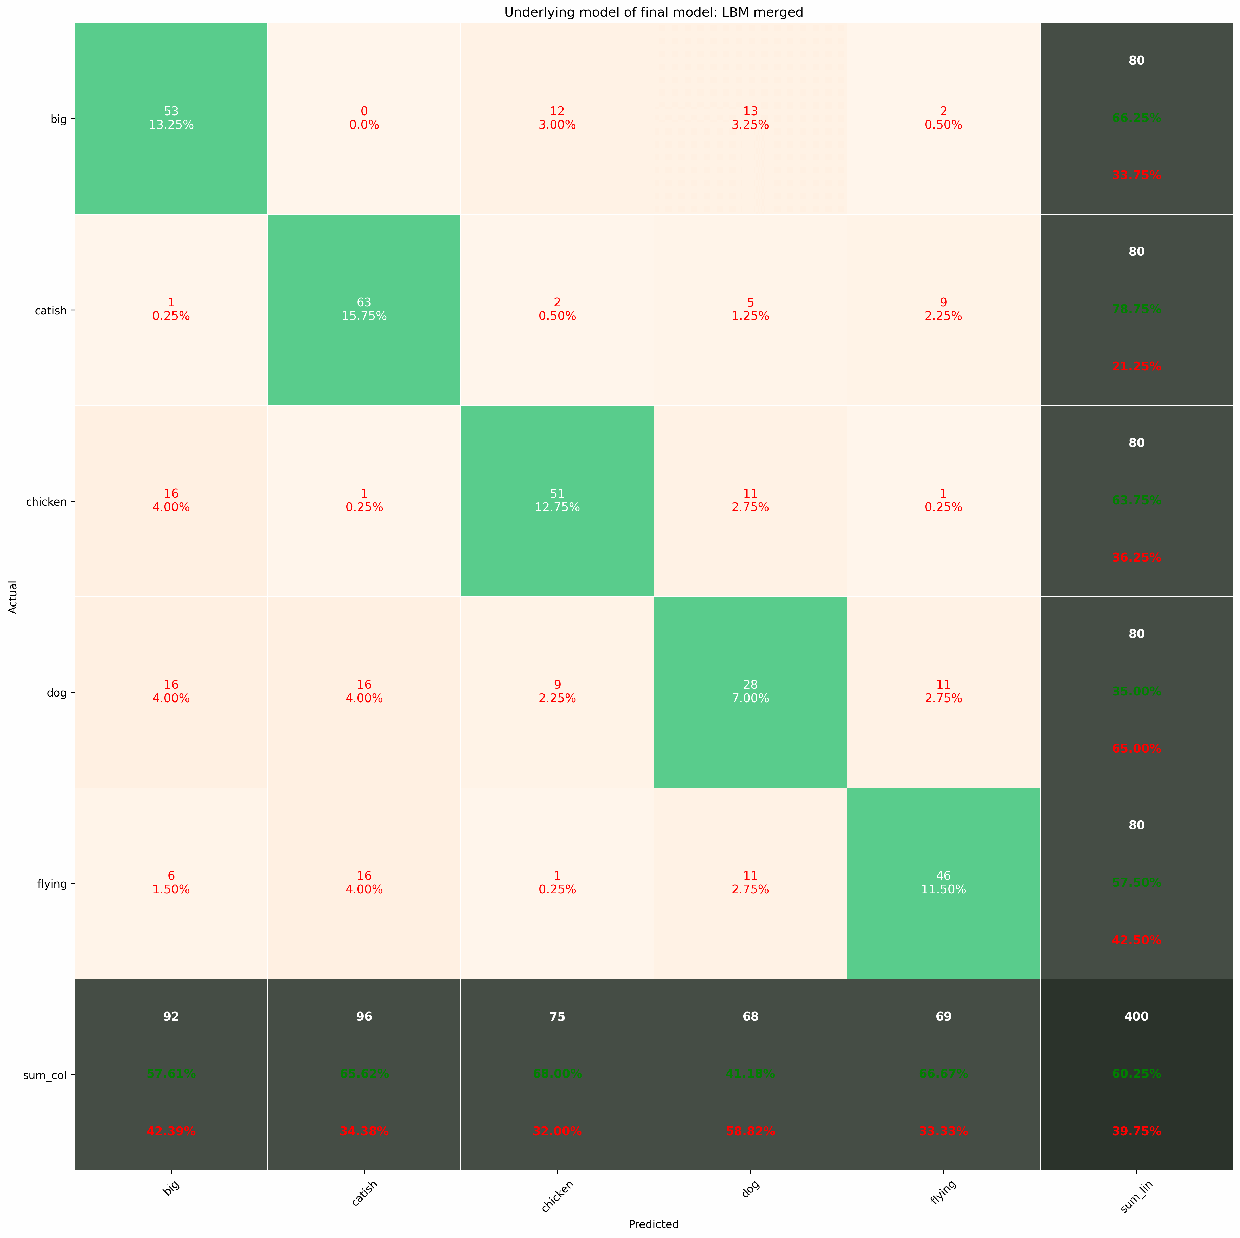
\includegraphics[width=\textwidth]{images/final/cm/underlying_LBM_merged.pdf}}
        \captionsetup{width=0.8\linewidth}
        \captionsetup{justification=centering}
        \caption{Underlying LBM model.}
    \end{subfigure}
    \hspace{1cm}
    \begin{subfigure}{.45\textwidth}
        \centering
        \fbox{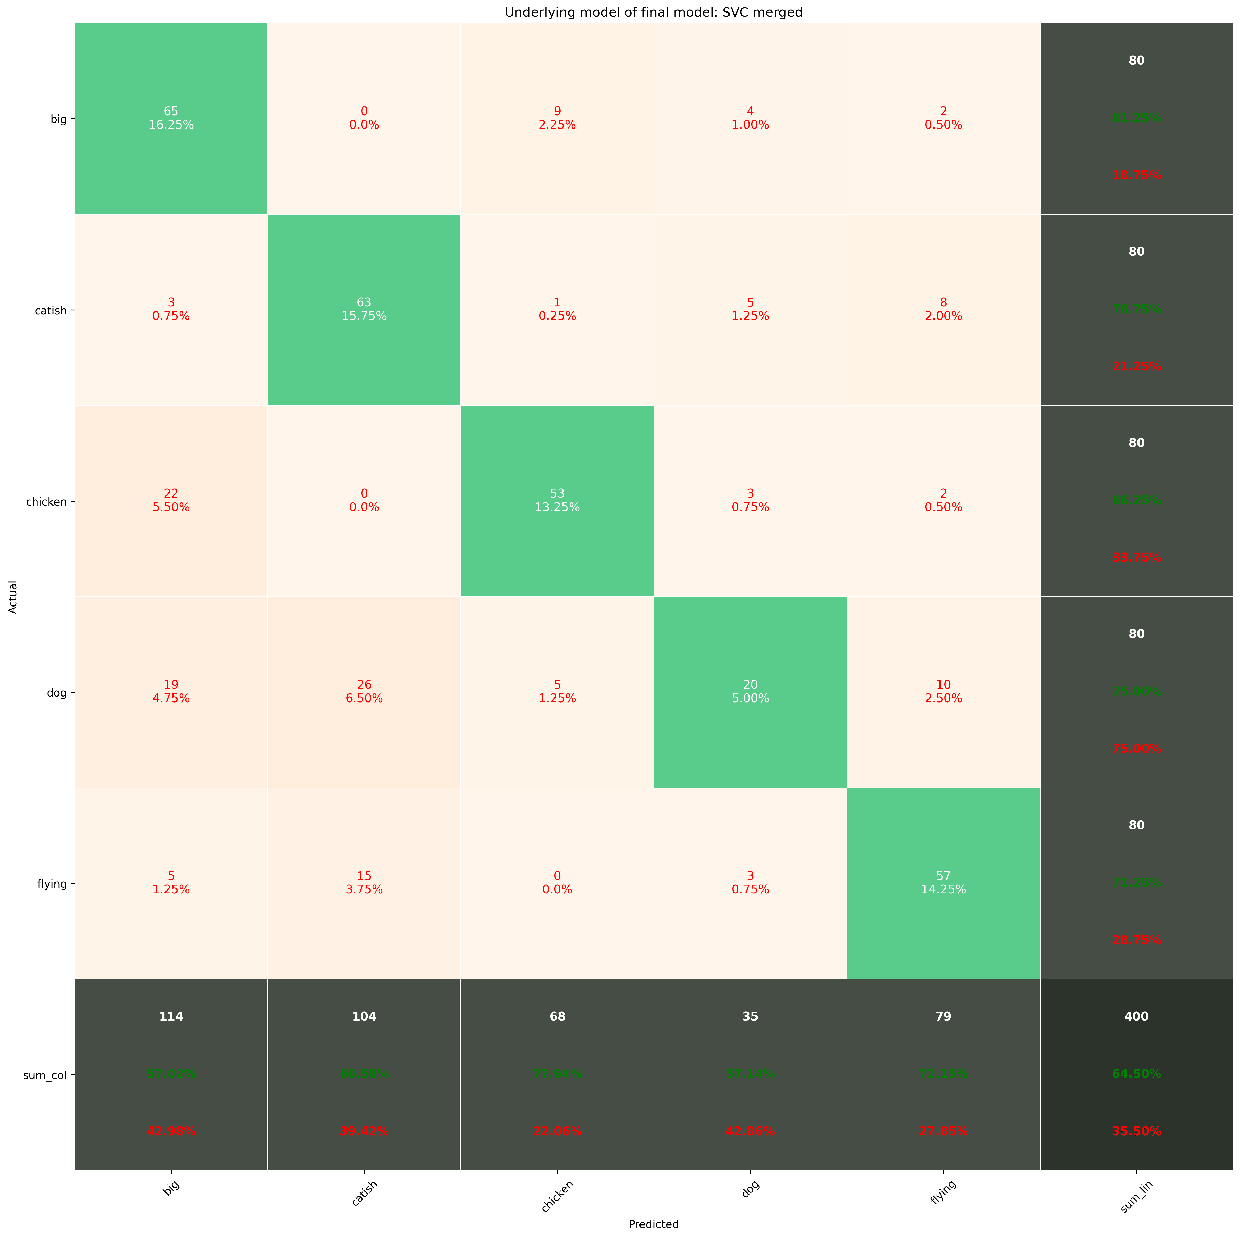
\includegraphics[width=\textwidth]{images/final/cm/underlying_SVC_merged.pdf}}
        \captionsetup{width=0.8\linewidth}
        \captionsetup{justification=centering}
        \caption{Underlying SVC model.}
    \end{subfigure}
    \captionsetup{width=0.9\linewidth}
    \captionsetup{justification=centering}
    \caption{Underlying models of the final model using the merged classes data set.}
\end{figure*}

\begin{figure*}[ht]
    \centering
    \begin{subfigure}{.45\textwidth}
        \centering
        \fbox{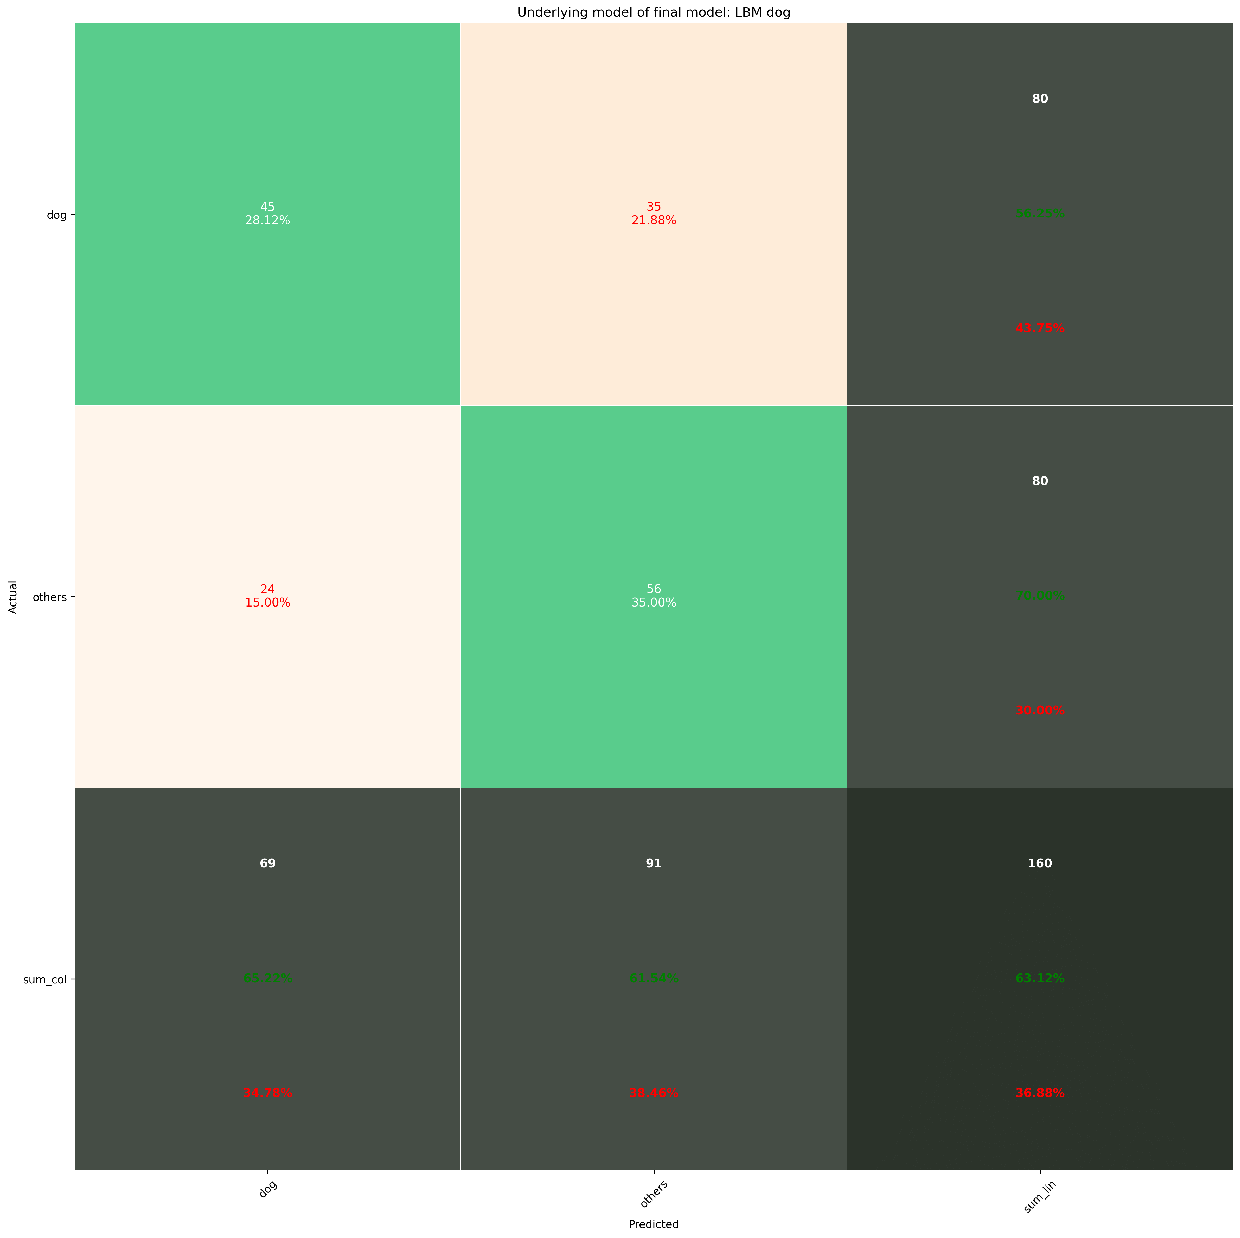
\includegraphics[width=\textwidth]{images/final/cm/underlying_LBM_dog.pdf}}
        \captionsetup{width=0.8\linewidth}
        \captionsetup{justification=centering}
        \caption{Underlying LBM model.}
    \end{subfigure}
    \hspace{1cm}
    \begin{subfigure}{.45\textwidth}
        \centering
        \fbox{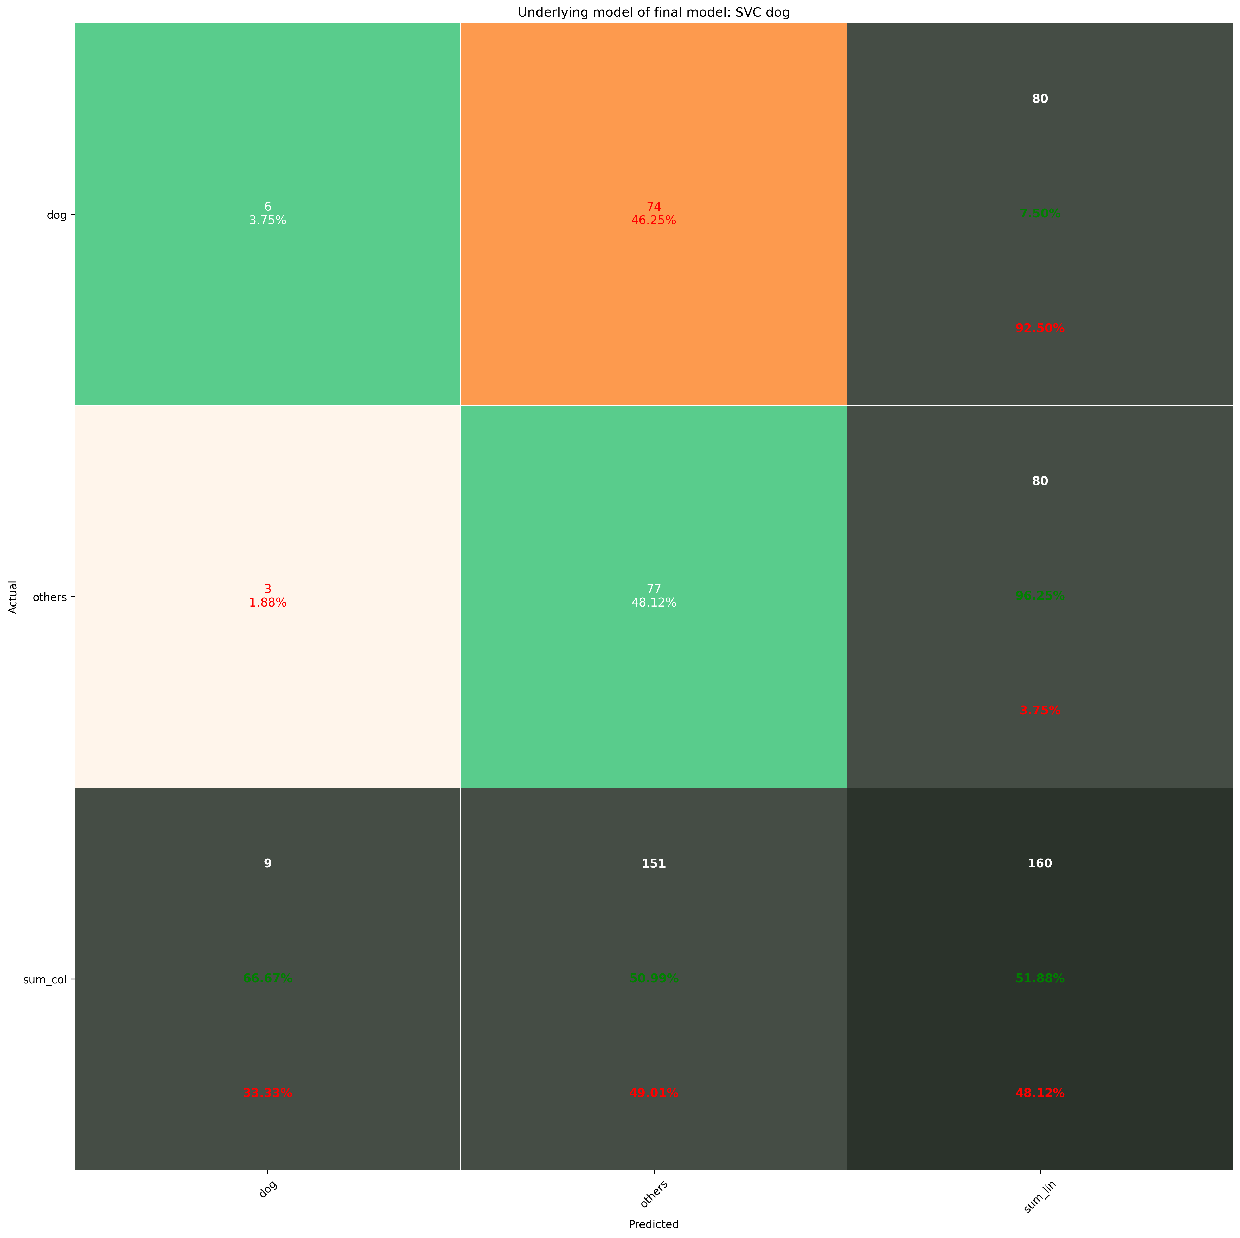
\includegraphics[width=\textwidth]{images/final/cm/underlying_SVC_dog.pdf}}
        \captionsetup{width=0.8\linewidth}
        \captionsetup{justification=centering}
        \caption{Underlying SVC model.}
    \end{subfigure}
    \captionsetup{width=0.9\linewidth}
    \captionsetup{justification=centering}
    \caption{Underlying models of the final model using the dogs vs others data set.}
\end{figure*}

\begin{figure*}[ht]
    \centering
    \begin{subfigure}{.45\textwidth}
        \centering
        \fbox{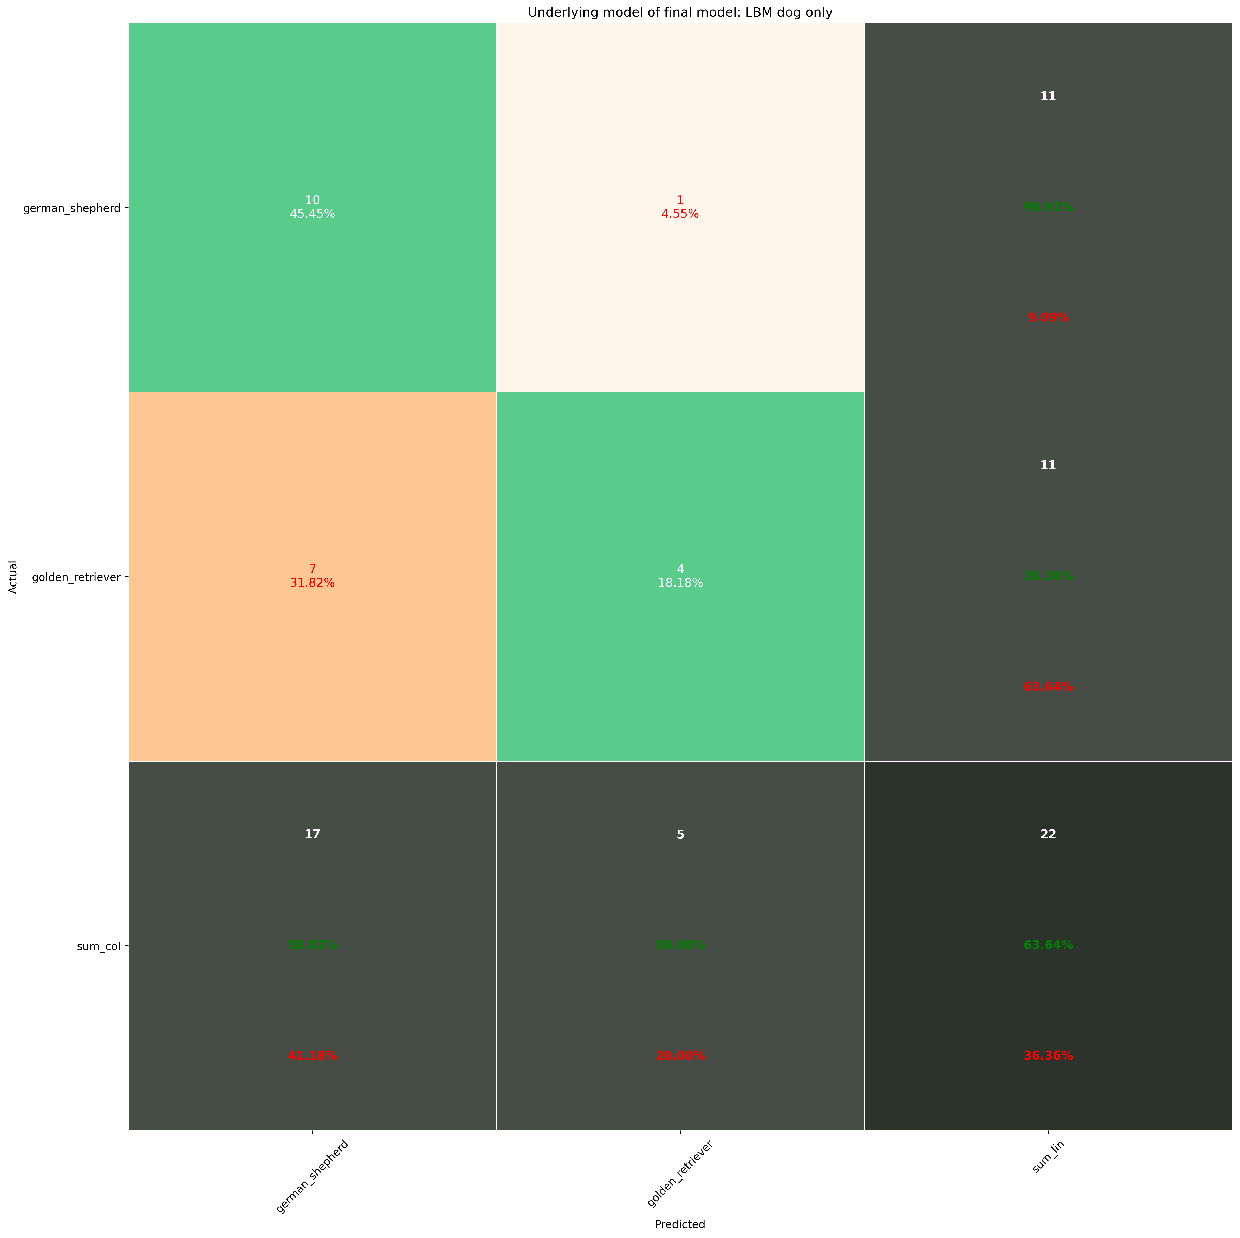
\includegraphics[width=\textwidth]{images/final/cm/underlying_LBM_dog_only.pdf}}
        \captionsetup{width=0.8\linewidth}
        \captionsetup{justification=centering}
        \caption{Underlying LBM sub-model.}
    \end{subfigure}
    \hspace{1cm}
    \begin{subfigure}{.45\textwidth}
        \centering
        \fbox{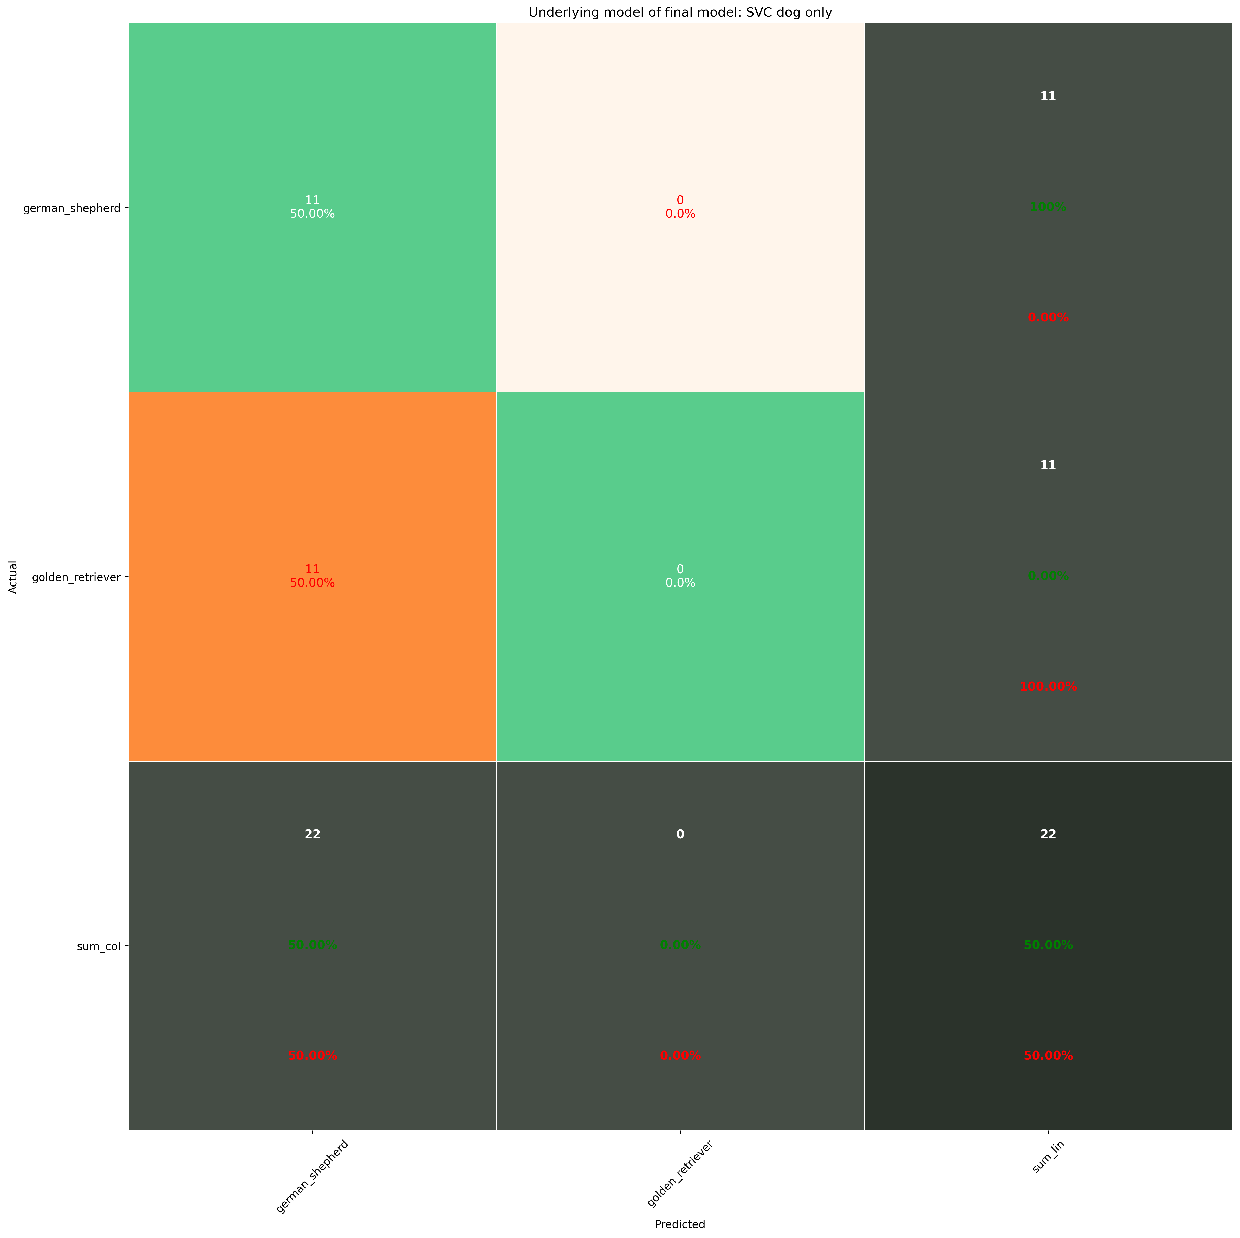
\includegraphics[width=\textwidth]{images/final/cm/underlying_SVC_dog_only.pdf}}
        \captionsetup{width=0.8\linewidth}
        \captionsetup{justification=centering}
        \caption{Underlying SVC sub-model.}
    \end{subfigure}
    \captionsetup{width=0.9\linewidth}
    \captionsetup{justification=centering}
    \caption{Underlying sub-models of the final model using a dog only split of the data set.}
\end{figure*}

\begin{figure*}[ht]
    \centering
    \begin{subfigure}{.45\textwidth}
        \centering
        \fbox{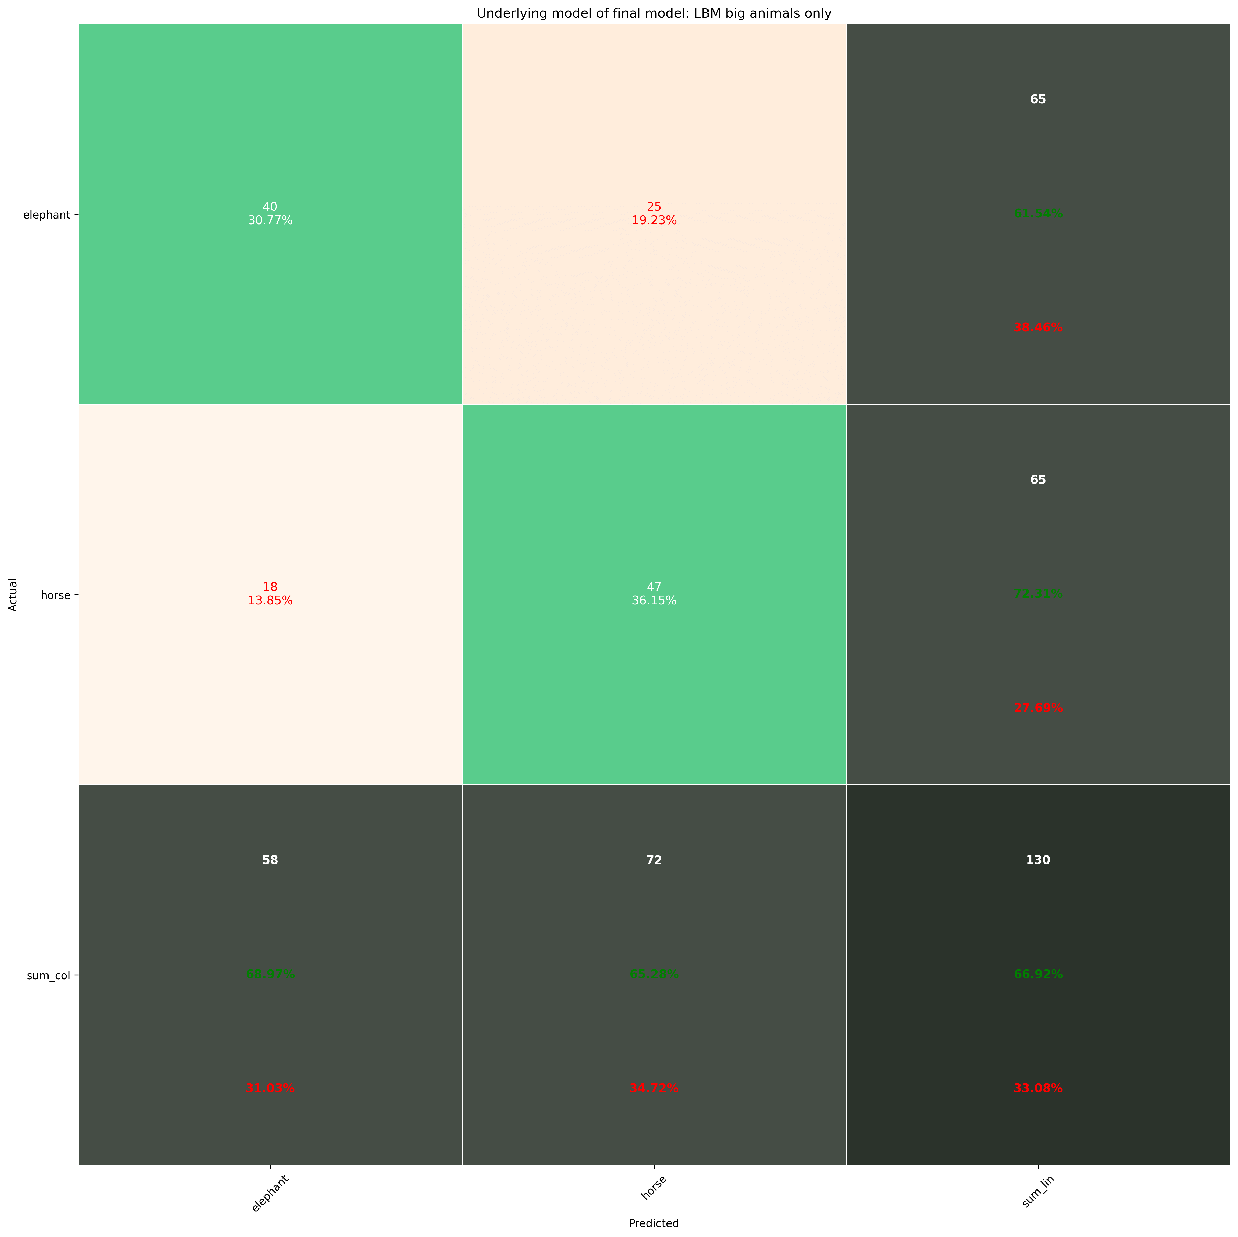
\includegraphics[width=\textwidth]{images/final/cm/underlying_LBM_big.pdf}}
        \captionsetup{width=0.8\linewidth}
        \captionsetup{justification=centering}
        \caption{Underlying LBM sub-model.}
    \end{subfigure}
    \hspace{1cm}
    \begin{subfigure}{.45\textwidth}
        \centering
        \fbox{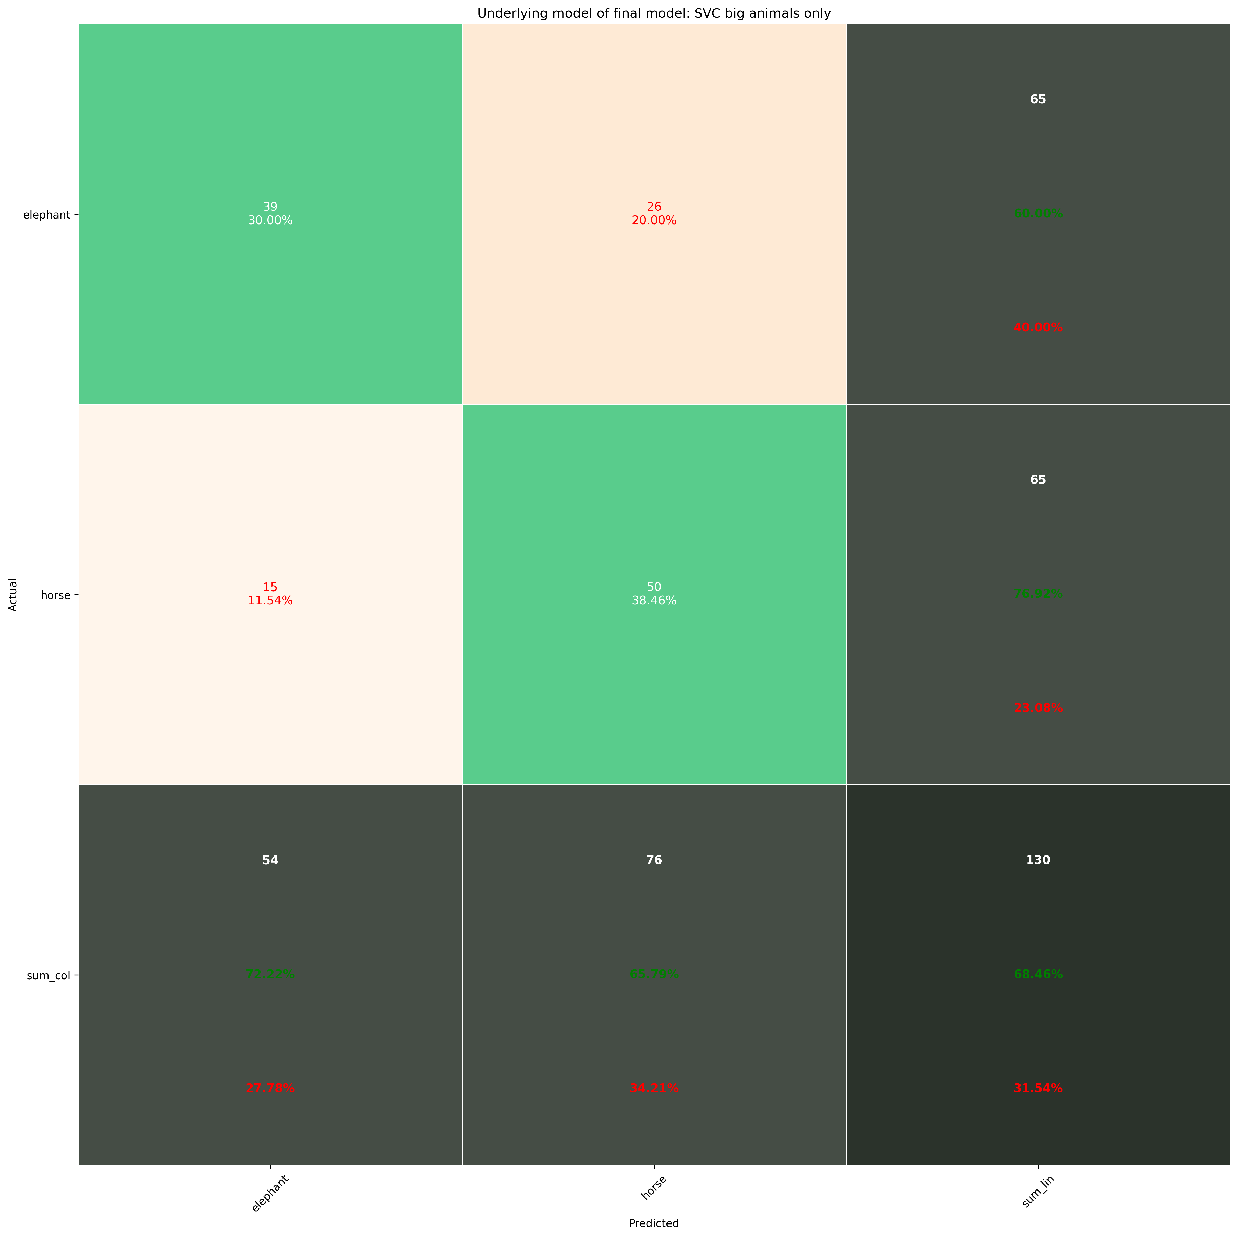
\includegraphics[width=\textwidth]{images/final/cm/underlying_SVC_big.pdf}}
        \captionsetup{width=0.8\linewidth}
        \captionsetup{justification=centering}
        \caption{Underlying SVC sub-model.}
    \end{subfigure}
    \captionsetup{width=0.9\linewidth}
    \captionsetup{justification=centering}
    \caption{Underlying sub-models of the final model using a \textit{big animals} split.}
\end{figure*}

\begin{figure*}[ht]
    \centering
    \begin{subfigure}{.45\textwidth}
        \centering
        \fbox{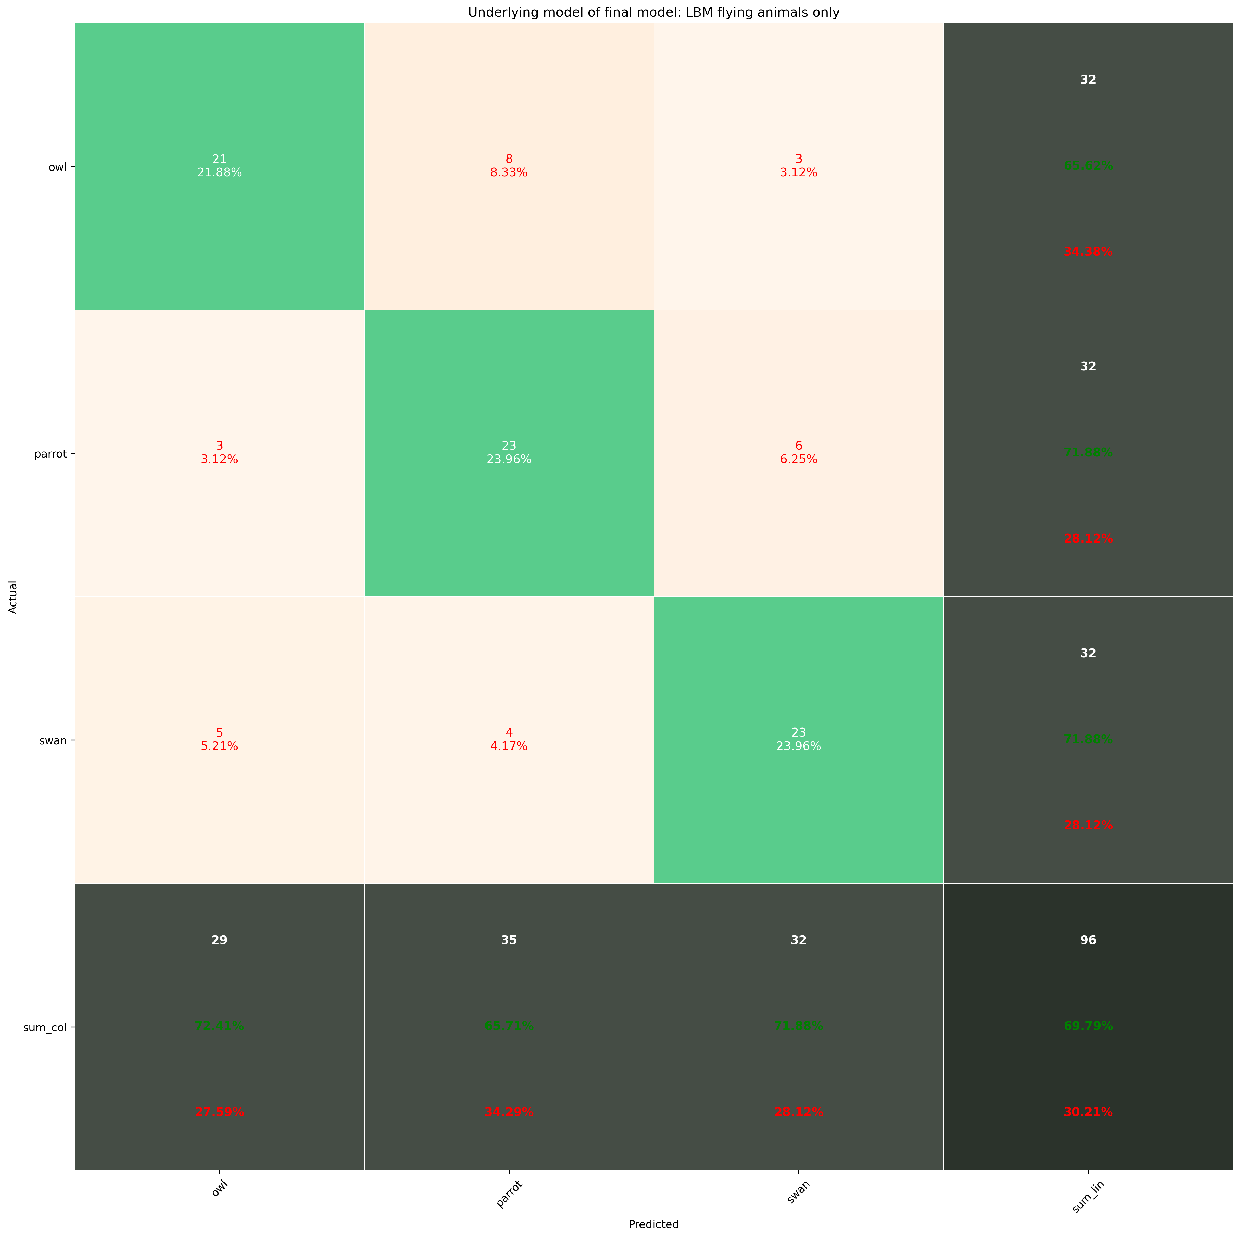
\includegraphics[width=\textwidth]{images/final/cm/underlying_LBM_flying.pdf}}
        \captionsetup{width=0.8\linewidth}
        \captionsetup{justification=centering}
        \caption{Underlying LBM sub-model.}
    \end{subfigure}
    \hspace{1cm}
    \begin{subfigure}{.45\textwidth}
        \centering
        \fbox{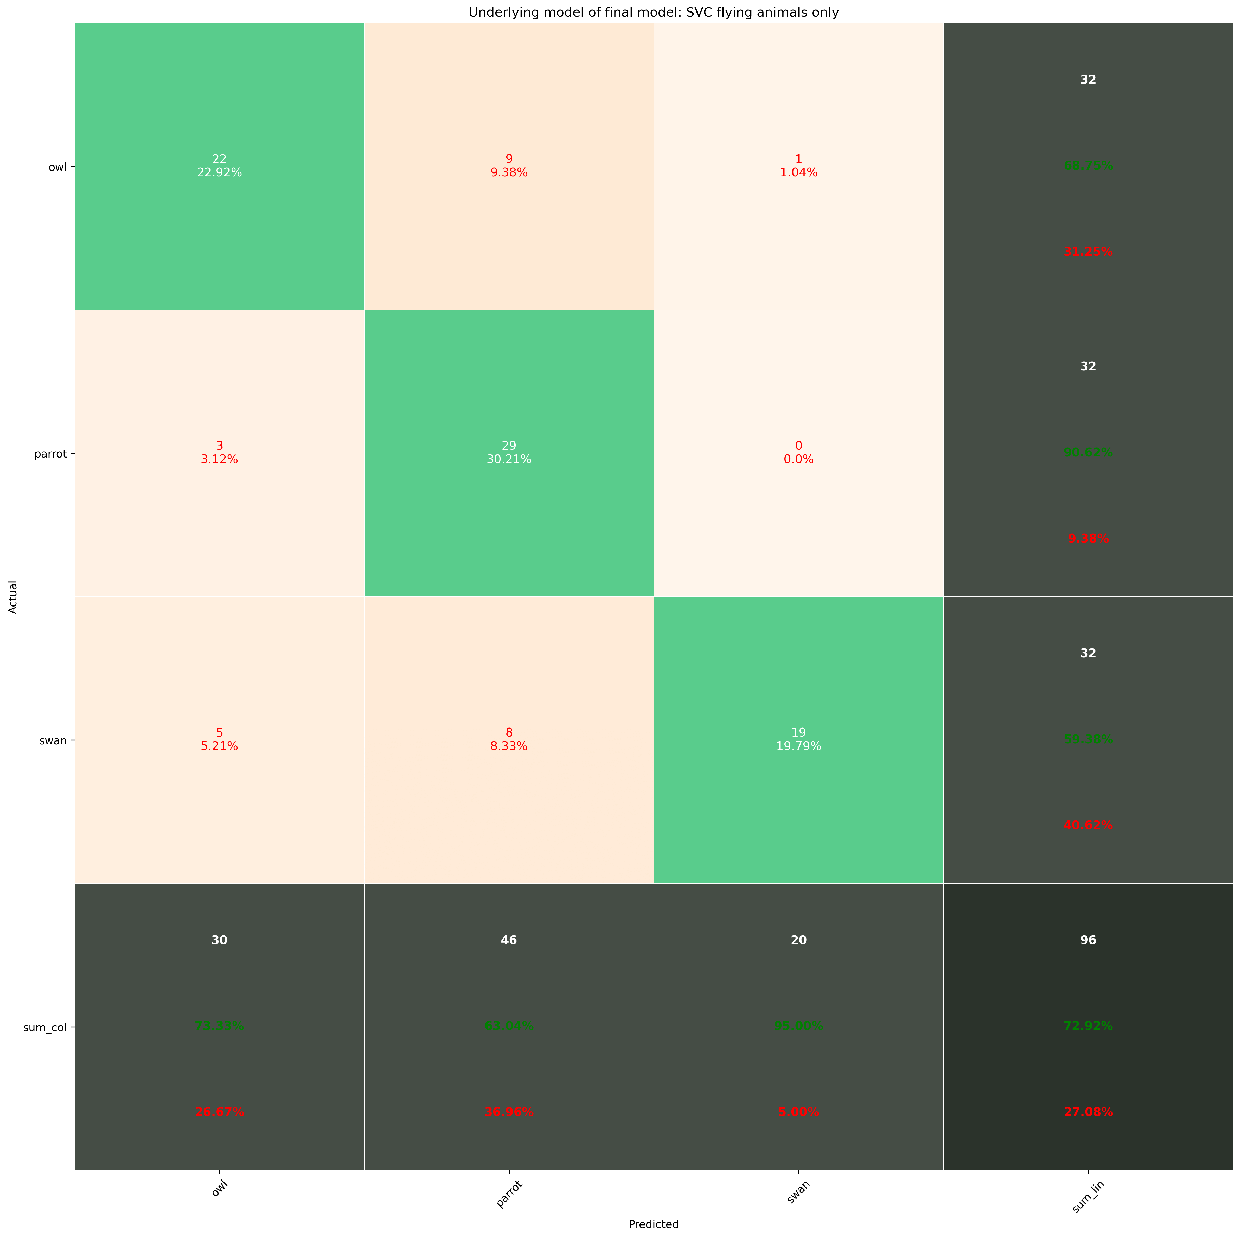
\includegraphics[width=\textwidth]{images/final/cm/underlying_SVC_flying.pdf}}
        \captionsetup{width=0.8\linewidth}
        \captionsetup{justification=centering}
        \caption{Underlying SVC sub-model.}
    \end{subfigure}
    \captionsetup{width=0.9\linewidth}
    \captionsetup{justification=centering}
    \caption{Underlying sub-models of the final model using a \textit{flying animals} split.}
\end{figure*}

\begin{figure*}[ht]
    \centering
    \begin{subfigure}{.45\textwidth}
        \centering
        \fbox{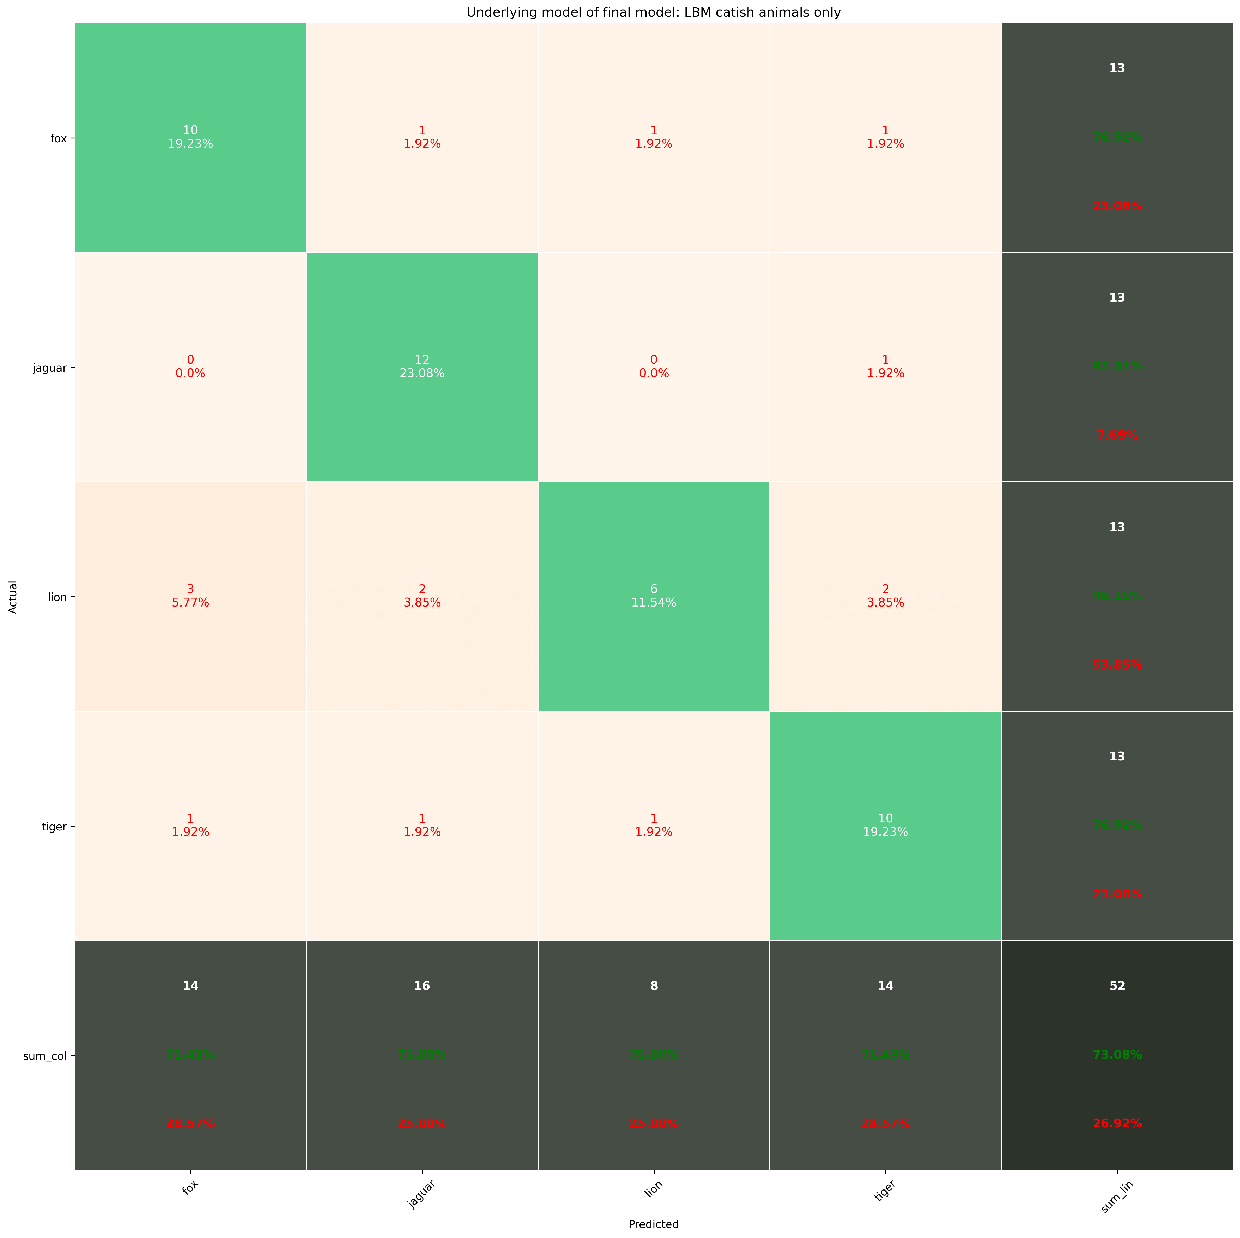
\includegraphics[width=\textwidth]{images/final/cm/underlying_LBM_catish.pdf}}
        \captionsetup{width=0.8\linewidth}
        \captionsetup{justification=centering}
        \caption{Underlying LBM sub-model.}
    \end{subfigure}
    \hspace{1cm}
    \begin{subfigure}{.45\textwidth}
        \centering
        \fbox{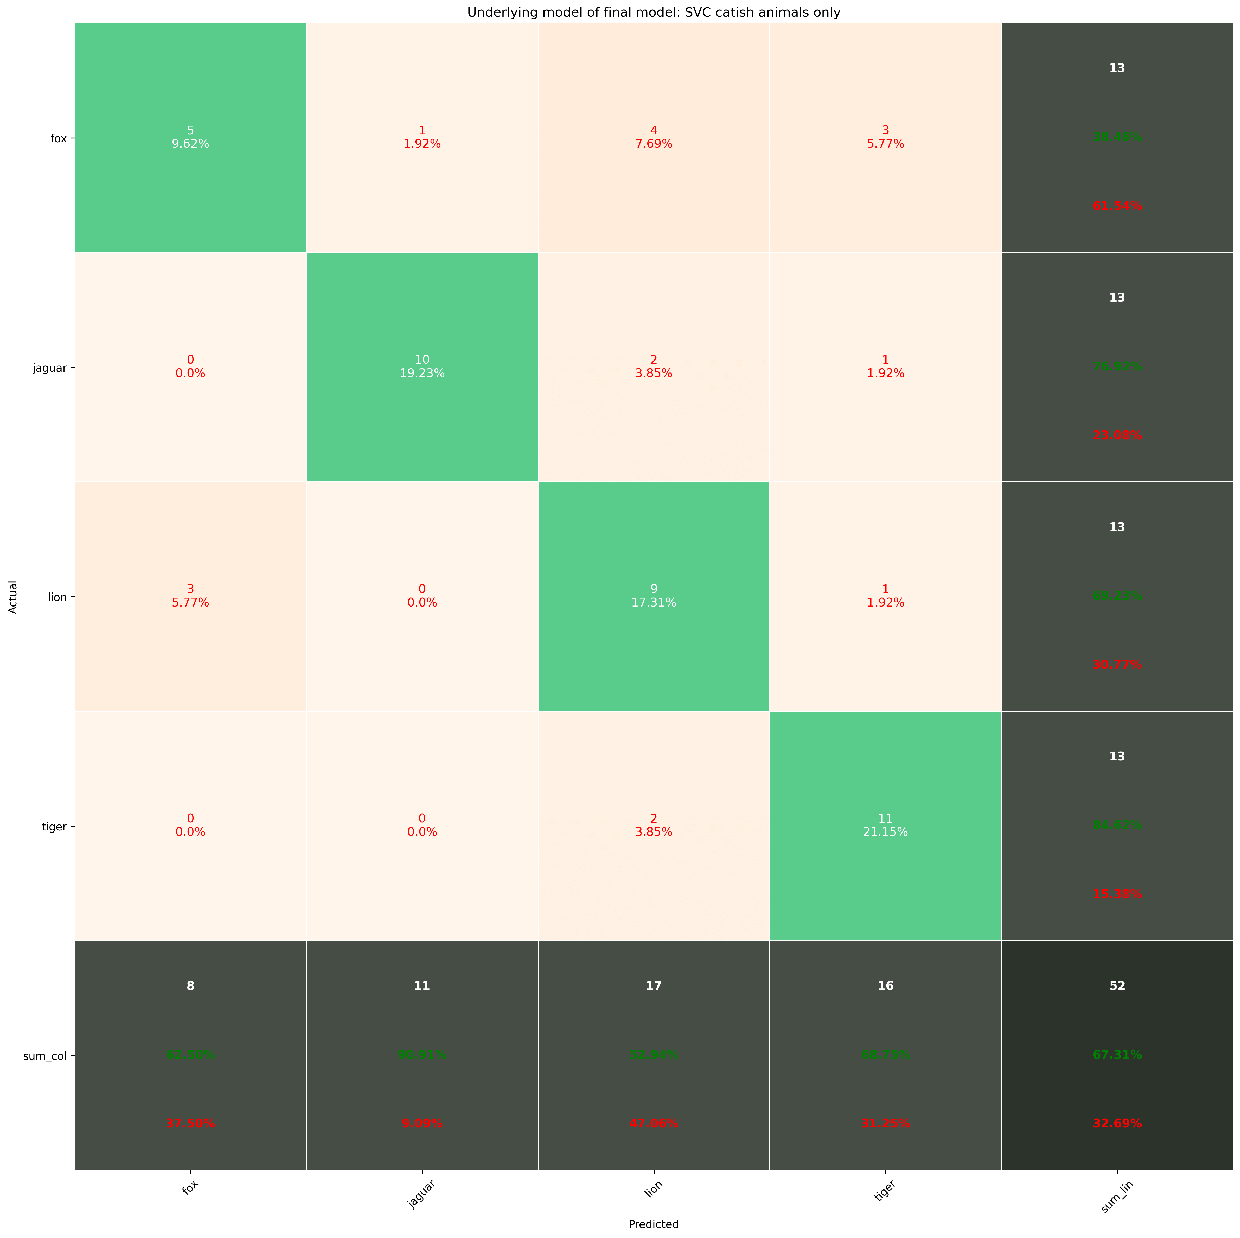
\includegraphics[width=\textwidth]{images/final/cm/underlying_SVC_catish.pdf}}
        \captionsetup{width=0.8\linewidth}
        \captionsetup{justification=centering}
        \caption{Underlying SVC sub-model.}
    \end{subfigure}
    \captionsetup{width=0.9\linewidth}
    \captionsetup{justification=centering}
    \caption{Underlying sub-models of the final model using a \textit{catish animals} split.}
\end{figure*}